\section{Presentation Logic Layer}

The web application is partially accessible to unauthenticated users, guests can visit the home page and the menu catalogue but any action that requires an account such as placing an order and accessing the dashboard redirects to the login page. The application exposes four JSP views, used for testing and developing purposes: ingredients, login, register and index (representation of the dashboard).
\subsection{Home Page}

The home page (figure \ref{fig:Home page's mockup}) is the entry point for all visitors. It presents a brief introduction to the service and provides navigation links to the login and registration pages. No authentication is required and if there are some meals available that day they are displayed in an overview-table.

\begin{figure}[H]
    \centering
    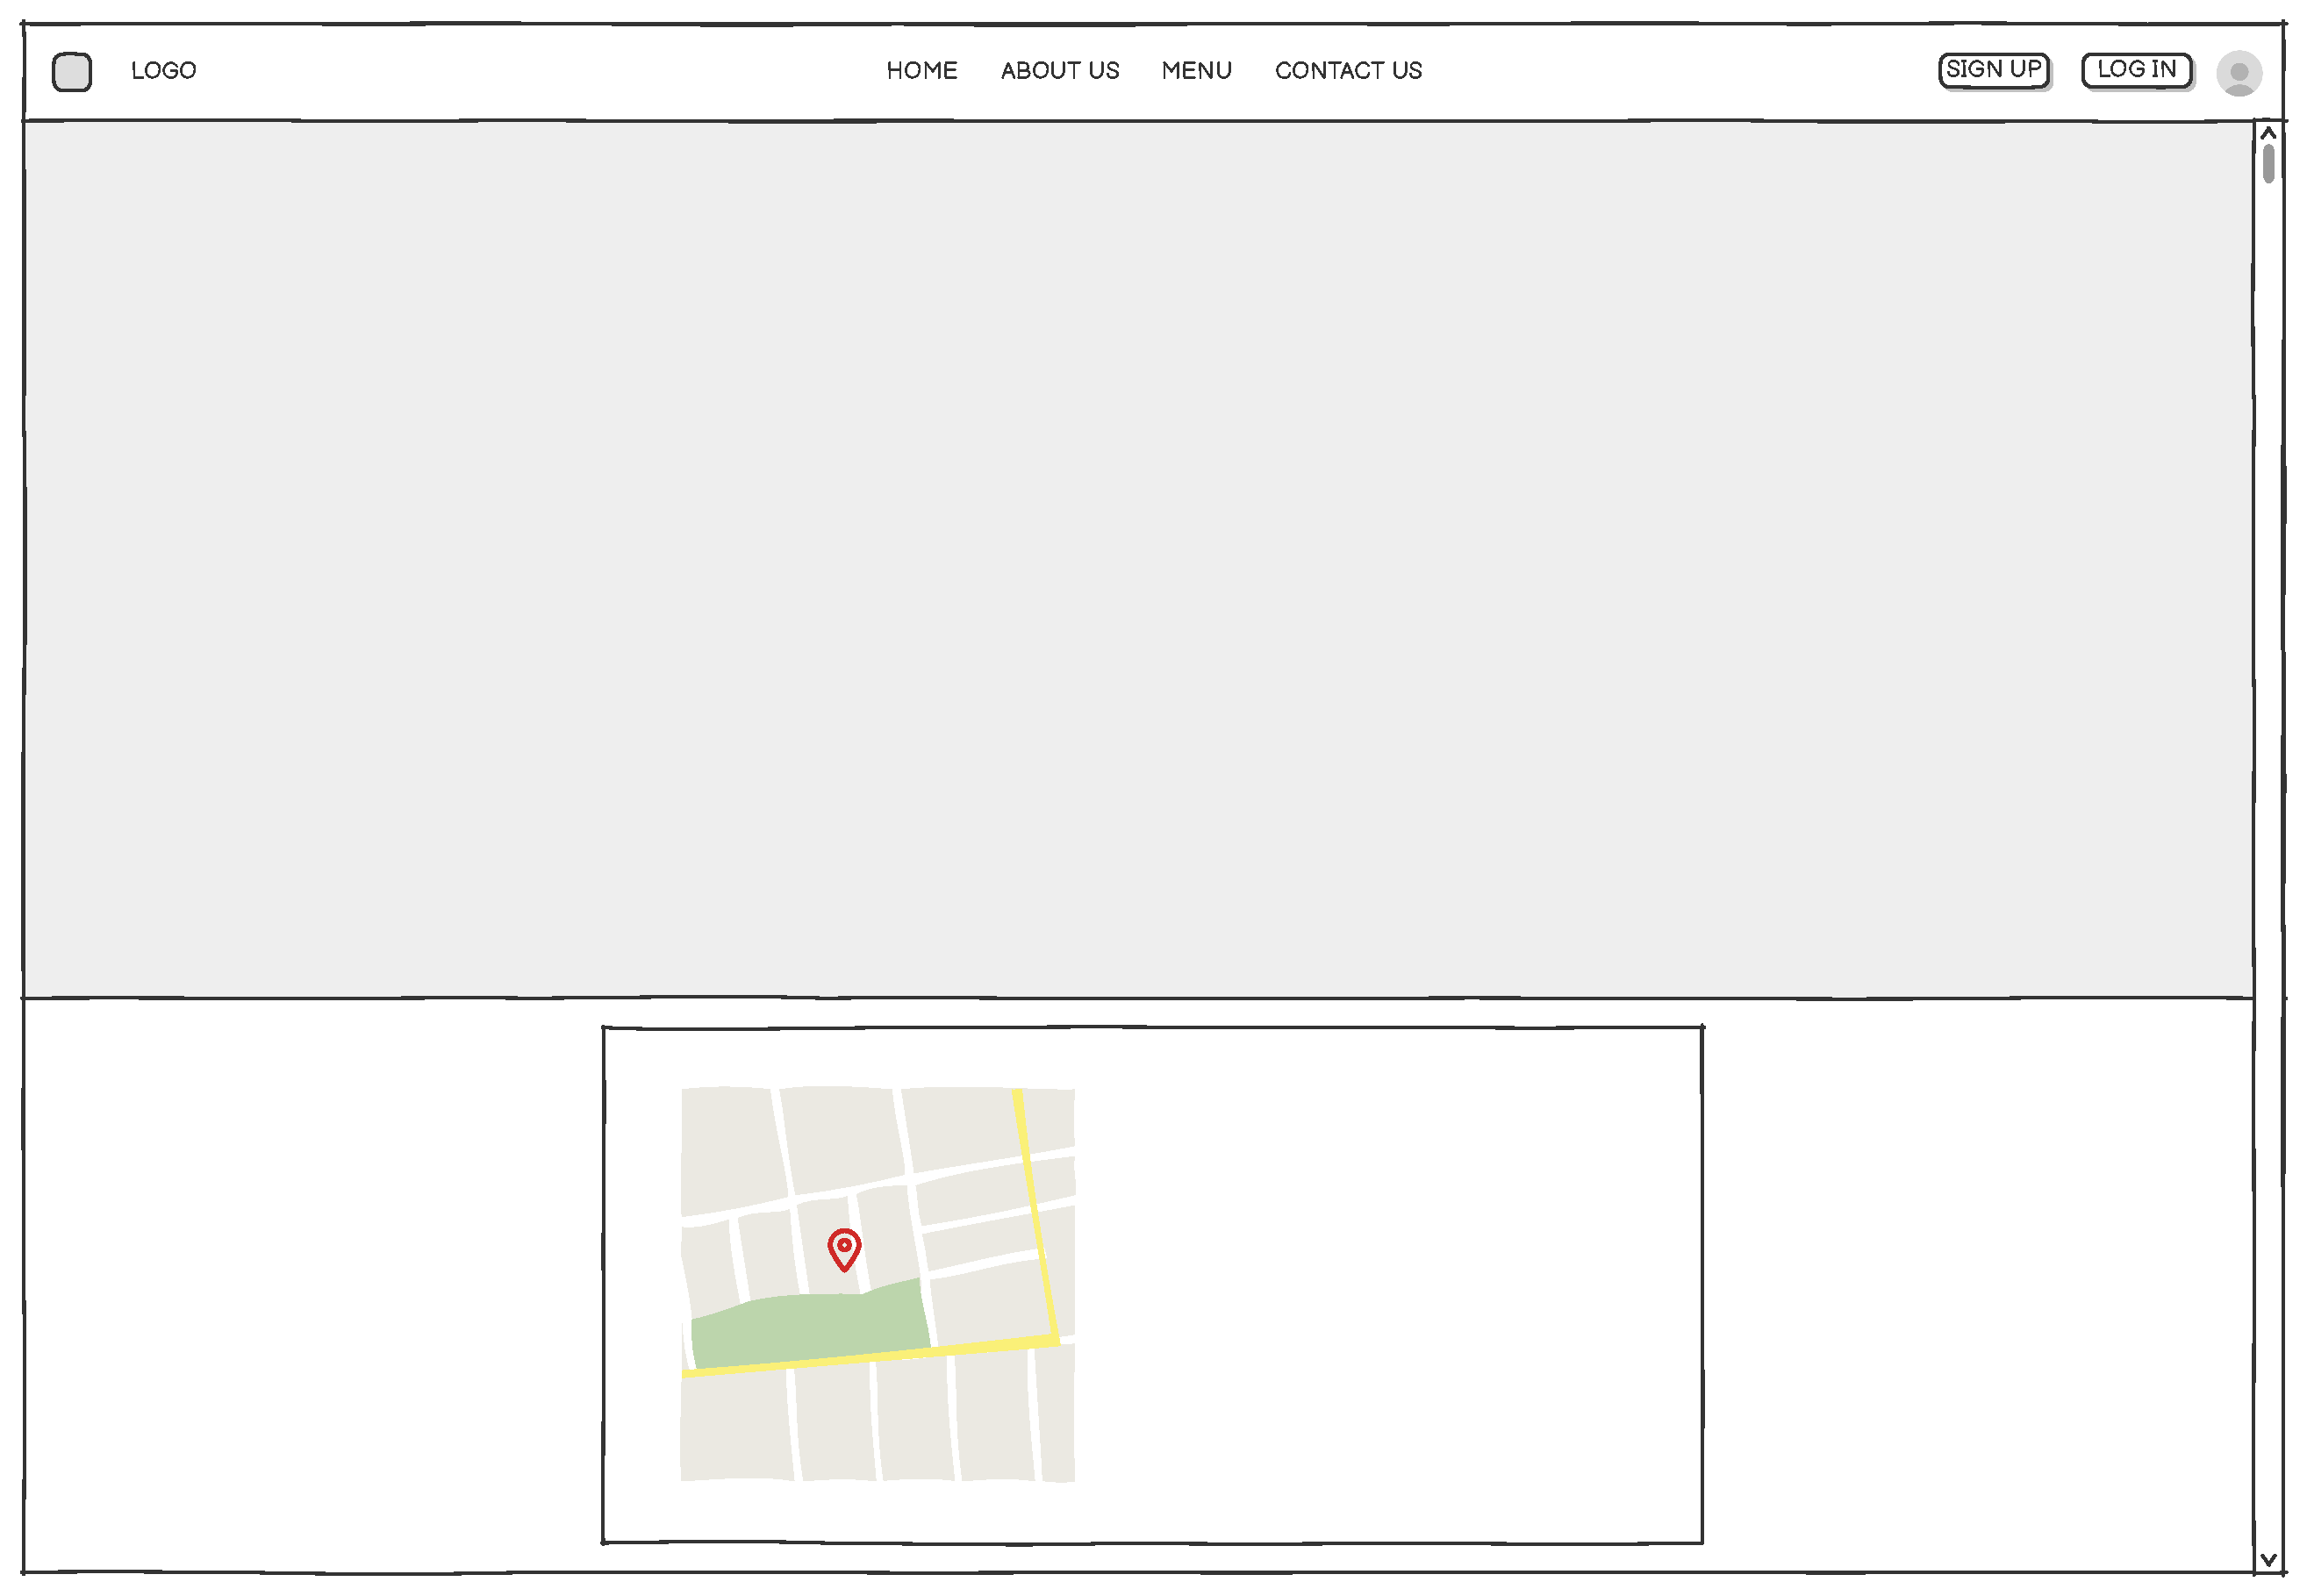
\includegraphics[width=0.9\textwidth]{images/Mockup/home.pdf}
    \caption{Home page's mockup}
    \label{fig:Home page's mockup}
\end{figure}


\subsection{Login Page}

The login page (figure \ref{fig:Log in's page mockup}) allows existing users to authenticate. The form collects the user's \textbf{email} and \textbf{password}. On submission, the credentials are sent via \texttt{POST /rest/user/login}. A successful login results in an \texttt{HttpOnly} cookie (\texttt{auth\_token}) containing a signed JWT and consequently the user is redirected to the dashboard. If authentication fails, an error message is displayed inline.

\begin{figure}[H]
    \centering
    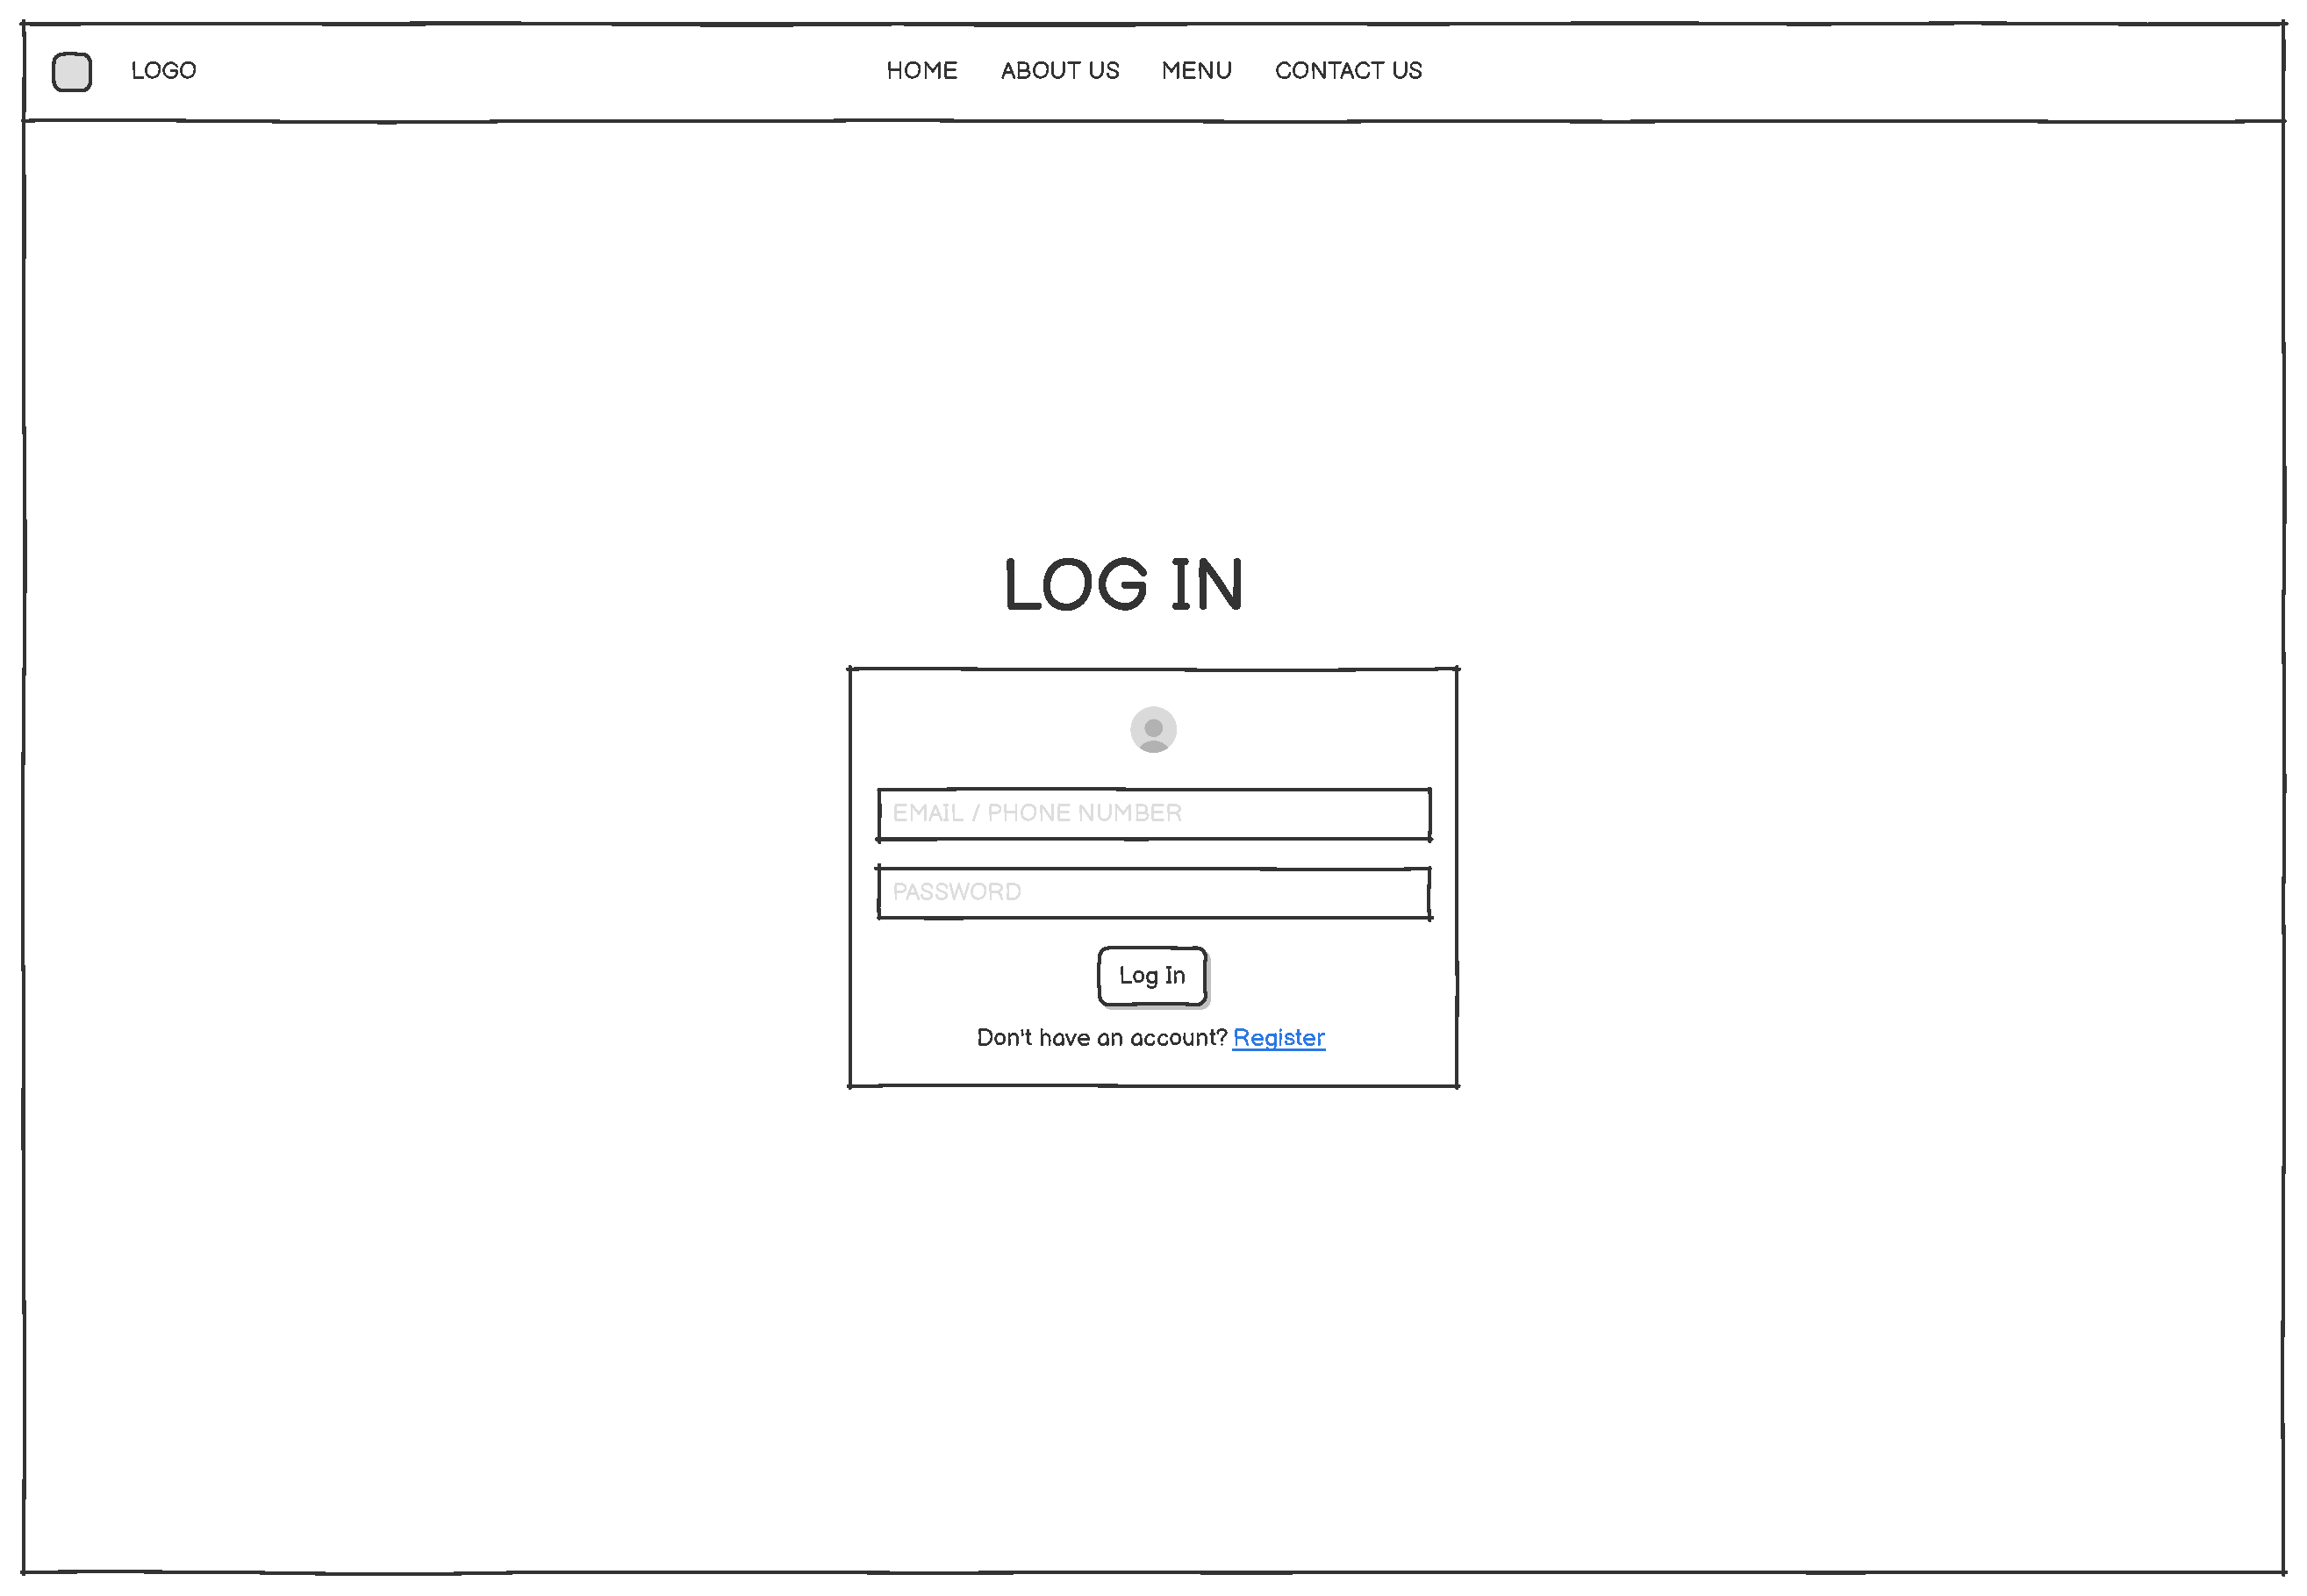
\includegraphics[width=0.9\textwidth]{images/Mockup/logIn.pdf}
    \caption{Log in's page mockup}
    \label{fig:Log in's page mockup}
\end{figure}


\subsection{Registration Page}

The registration page (figure \ref{fig:Example of compilation of registration's page mockup}) allows new customers to create an account. The form collects the following fields: \textbf{username}, \textbf{email}, \textbf{name}, \textbf{surname}, \textbf{phone number}, and \textbf{password}. All fields are mandatory so the user can't go on with the registration until all of them are filled. The password must satisfy a security policy: 8-16 characters, at least one uppercase letter, one lowercase letter, one digit and one special character. This policy is enforced server-side by the \texttt{Validator} utility class.
\texttt{Validator} utility class validates also the email field: it allows the first part of the e-mail address to contain one or more characters (letters, digits and symbols + \_ . -), followed by an @, a valid domain name, a dot and a top-level domain of at least two letters. On successful registration the user is redirected to the login page.

\begin{figure}[H]
    \centering
    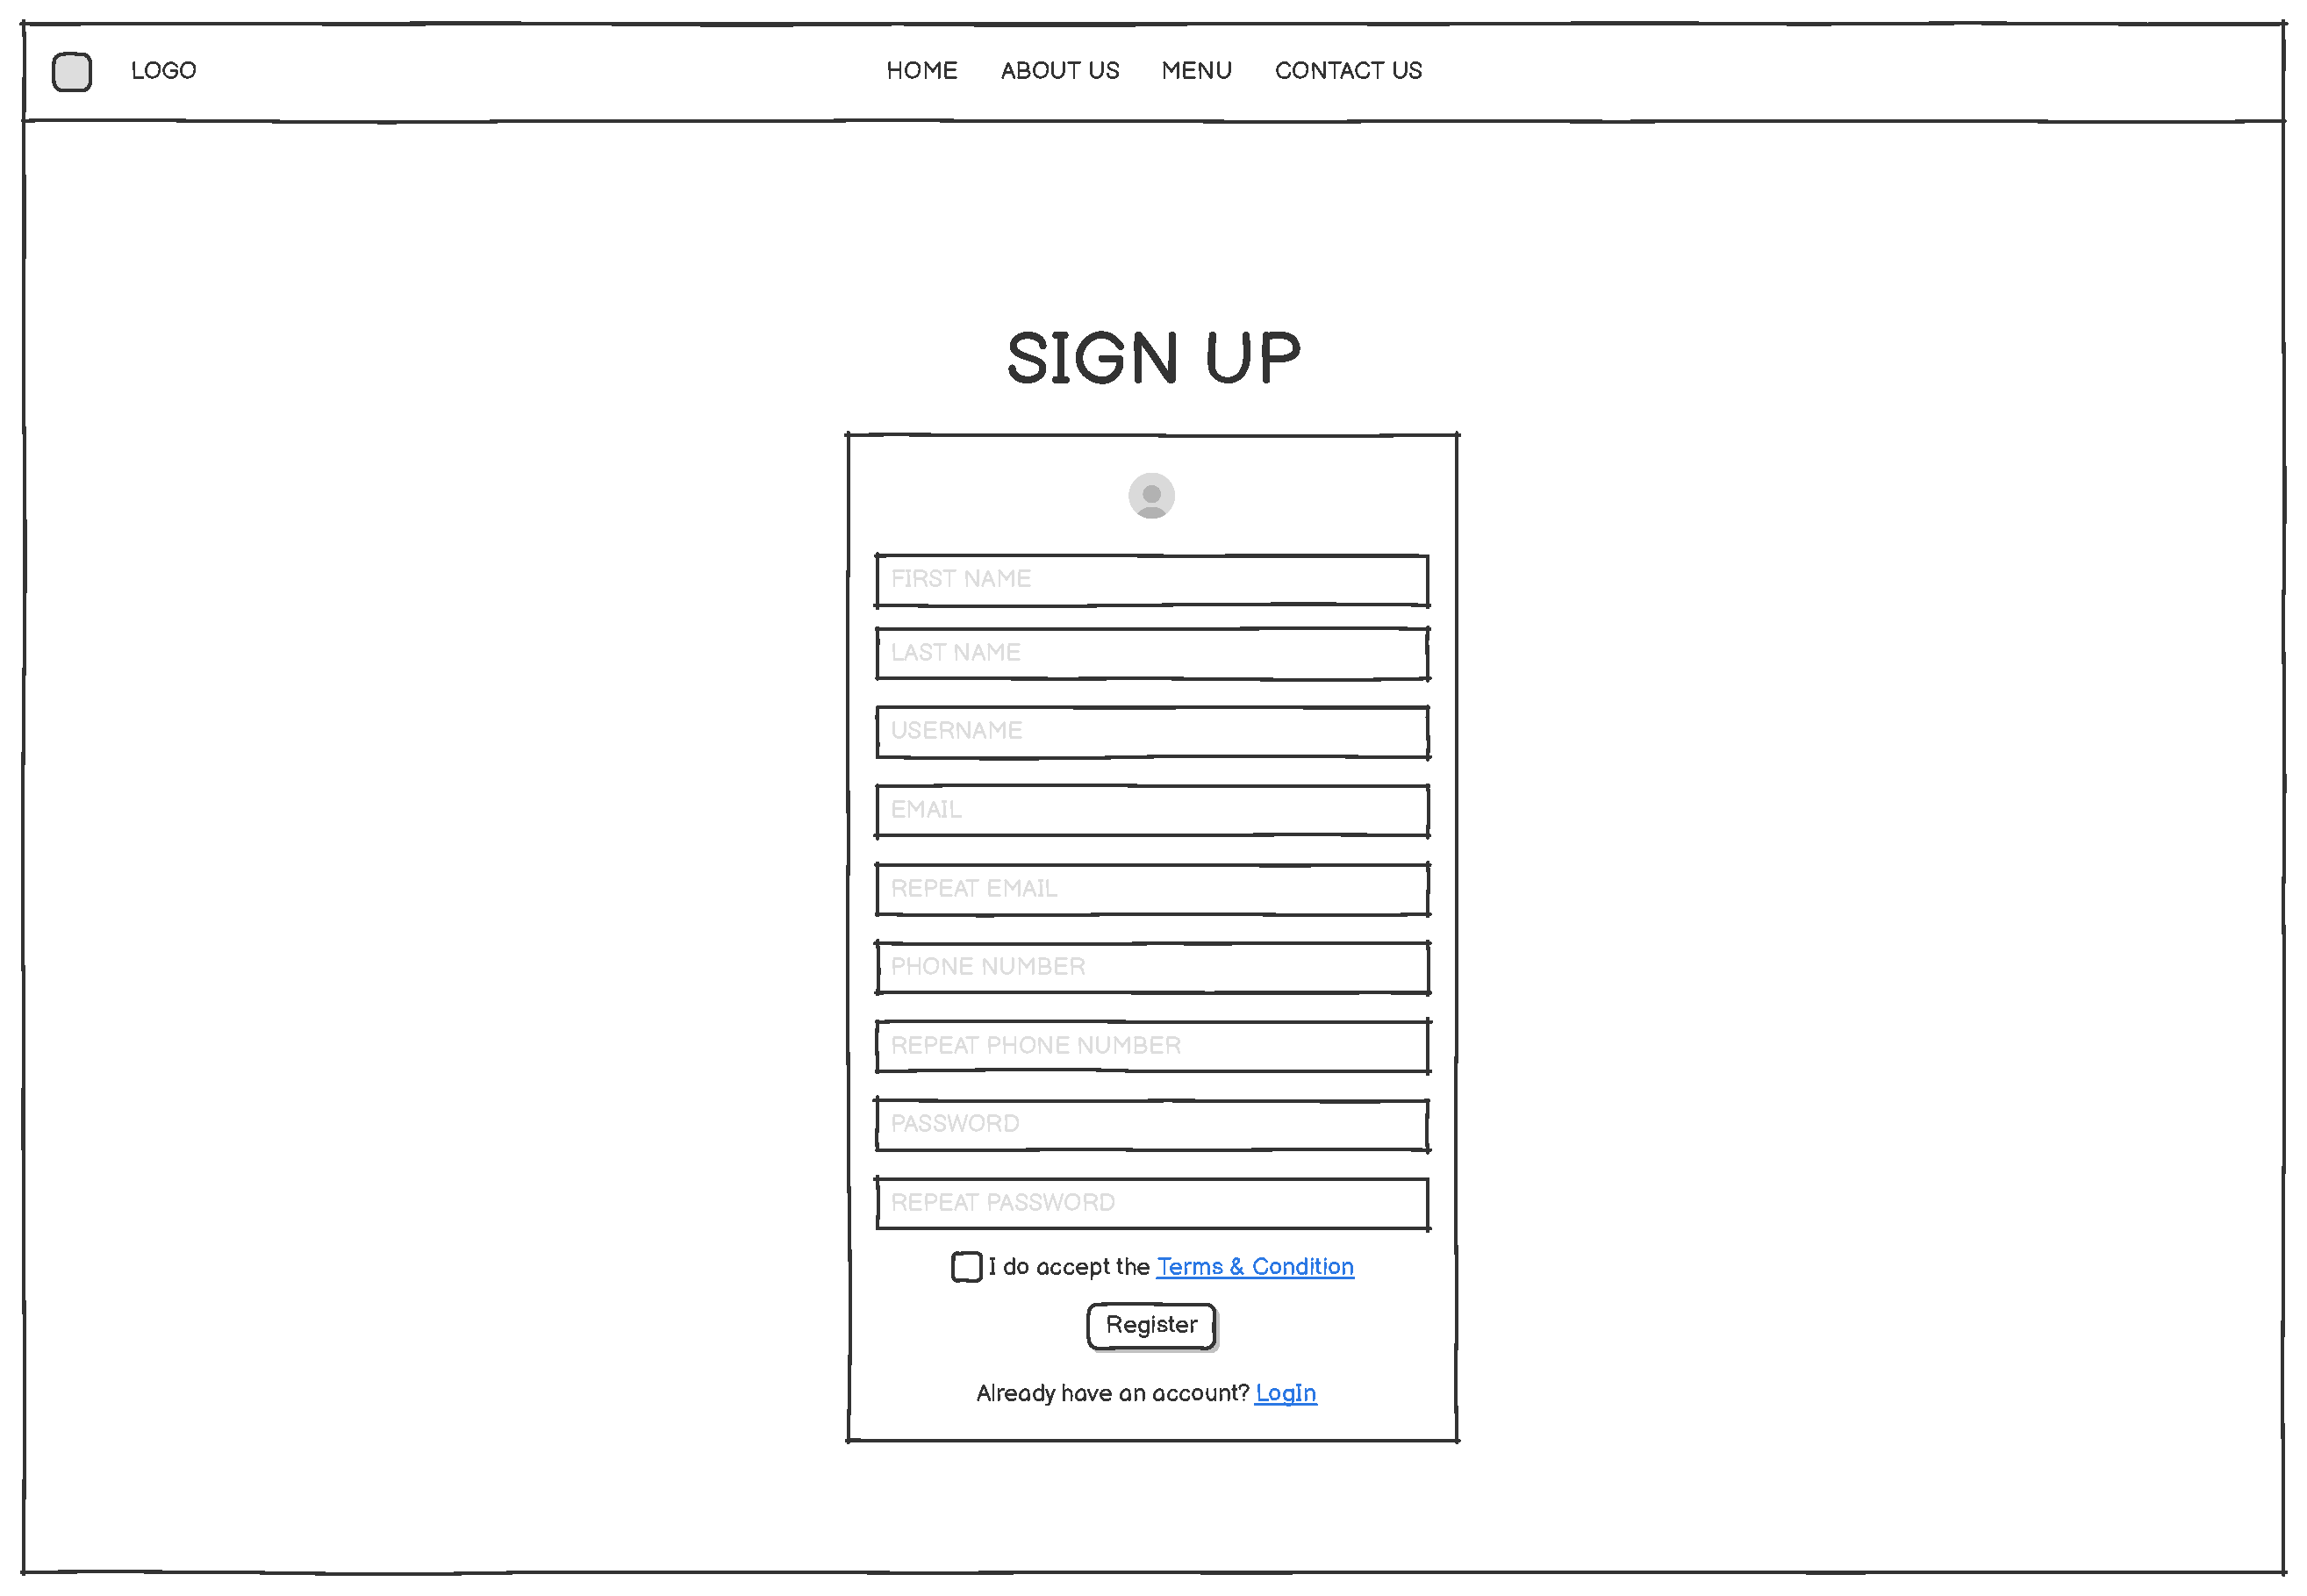
\includegraphics[width=0.9\textwidth]{images/Mockup/registration.pdf}
    \caption{Example of compilation of registration's page mockup}
    \label{fig:Example of compilation of registration's page mockup}
\end{figure}


\subsection{Dashboard}
The dashboard (figures \ref{fig:Management admin-side dishes dashboard mockup page.} - \ref{fig:Management staff-side dishes dashboard mockup page.} - \ref{fig:Dish's ingredients admin-side mockup page.} - \ref{fig:Dish's ingredients staff-side mockup page.} - \ref{fig:Menu dashboard's mockup page.}) is the main interface for authenticated users. The \texttt{AuthFilter} servlet filter is designed to protect all routes under \texttt{/dashboard/*} by validating the \texttt{auth\_token} HttpOnly cookie on every request. If the token is missing or expired, it redirects to \texttt{/login} otherwise it sets the \texttt{user\_id} request attribute. The dashboard will expose the menu catalogue, order management and staff/admin back-office functionality depending on the role of the authenticated user (\texttt{CUSTOMER}, \texttt{STAFF}, or \texttt{ADMIN}).
\begin{figure}[H]
    \centering
    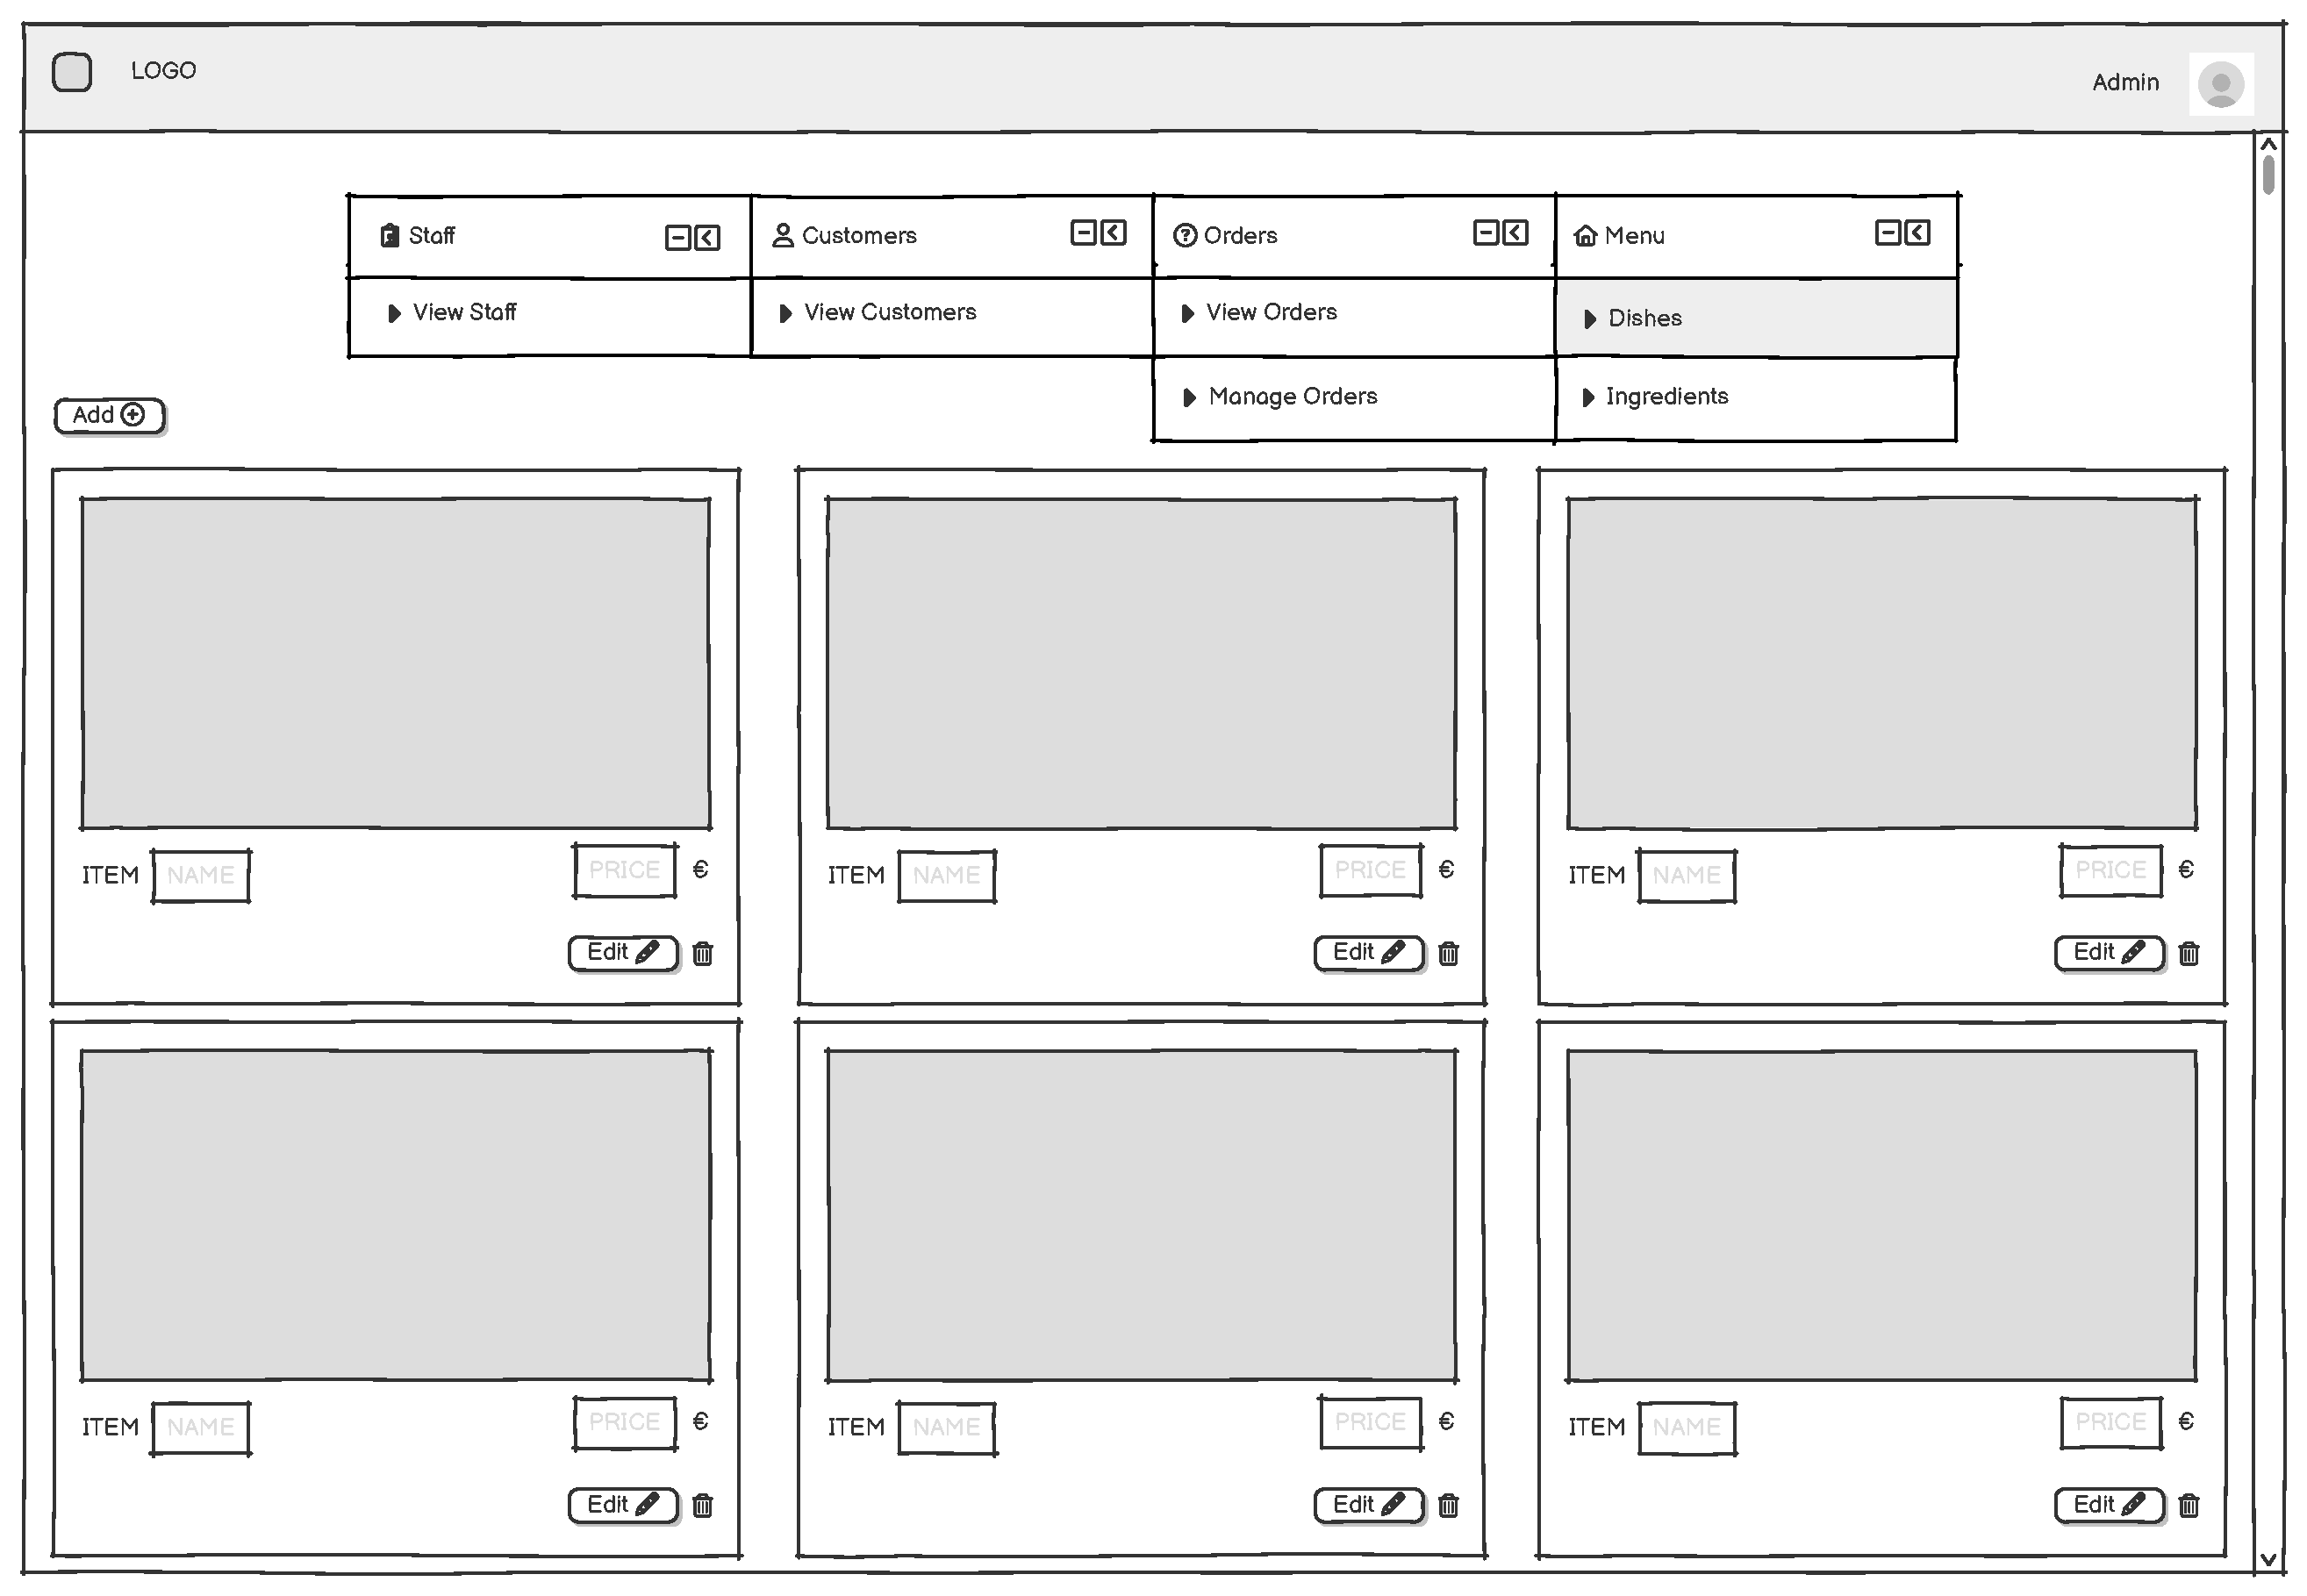
\includegraphics[width=0.8\textwidth]{images/Mockup/adminDishesList.pdf}
    \caption{Management admin-side dishes dashboard mockup page.}
    \label{fig:Management admin-side dishes dashboard mockup page.}
\end{figure}

\begin{figure}[H]
    \centering
    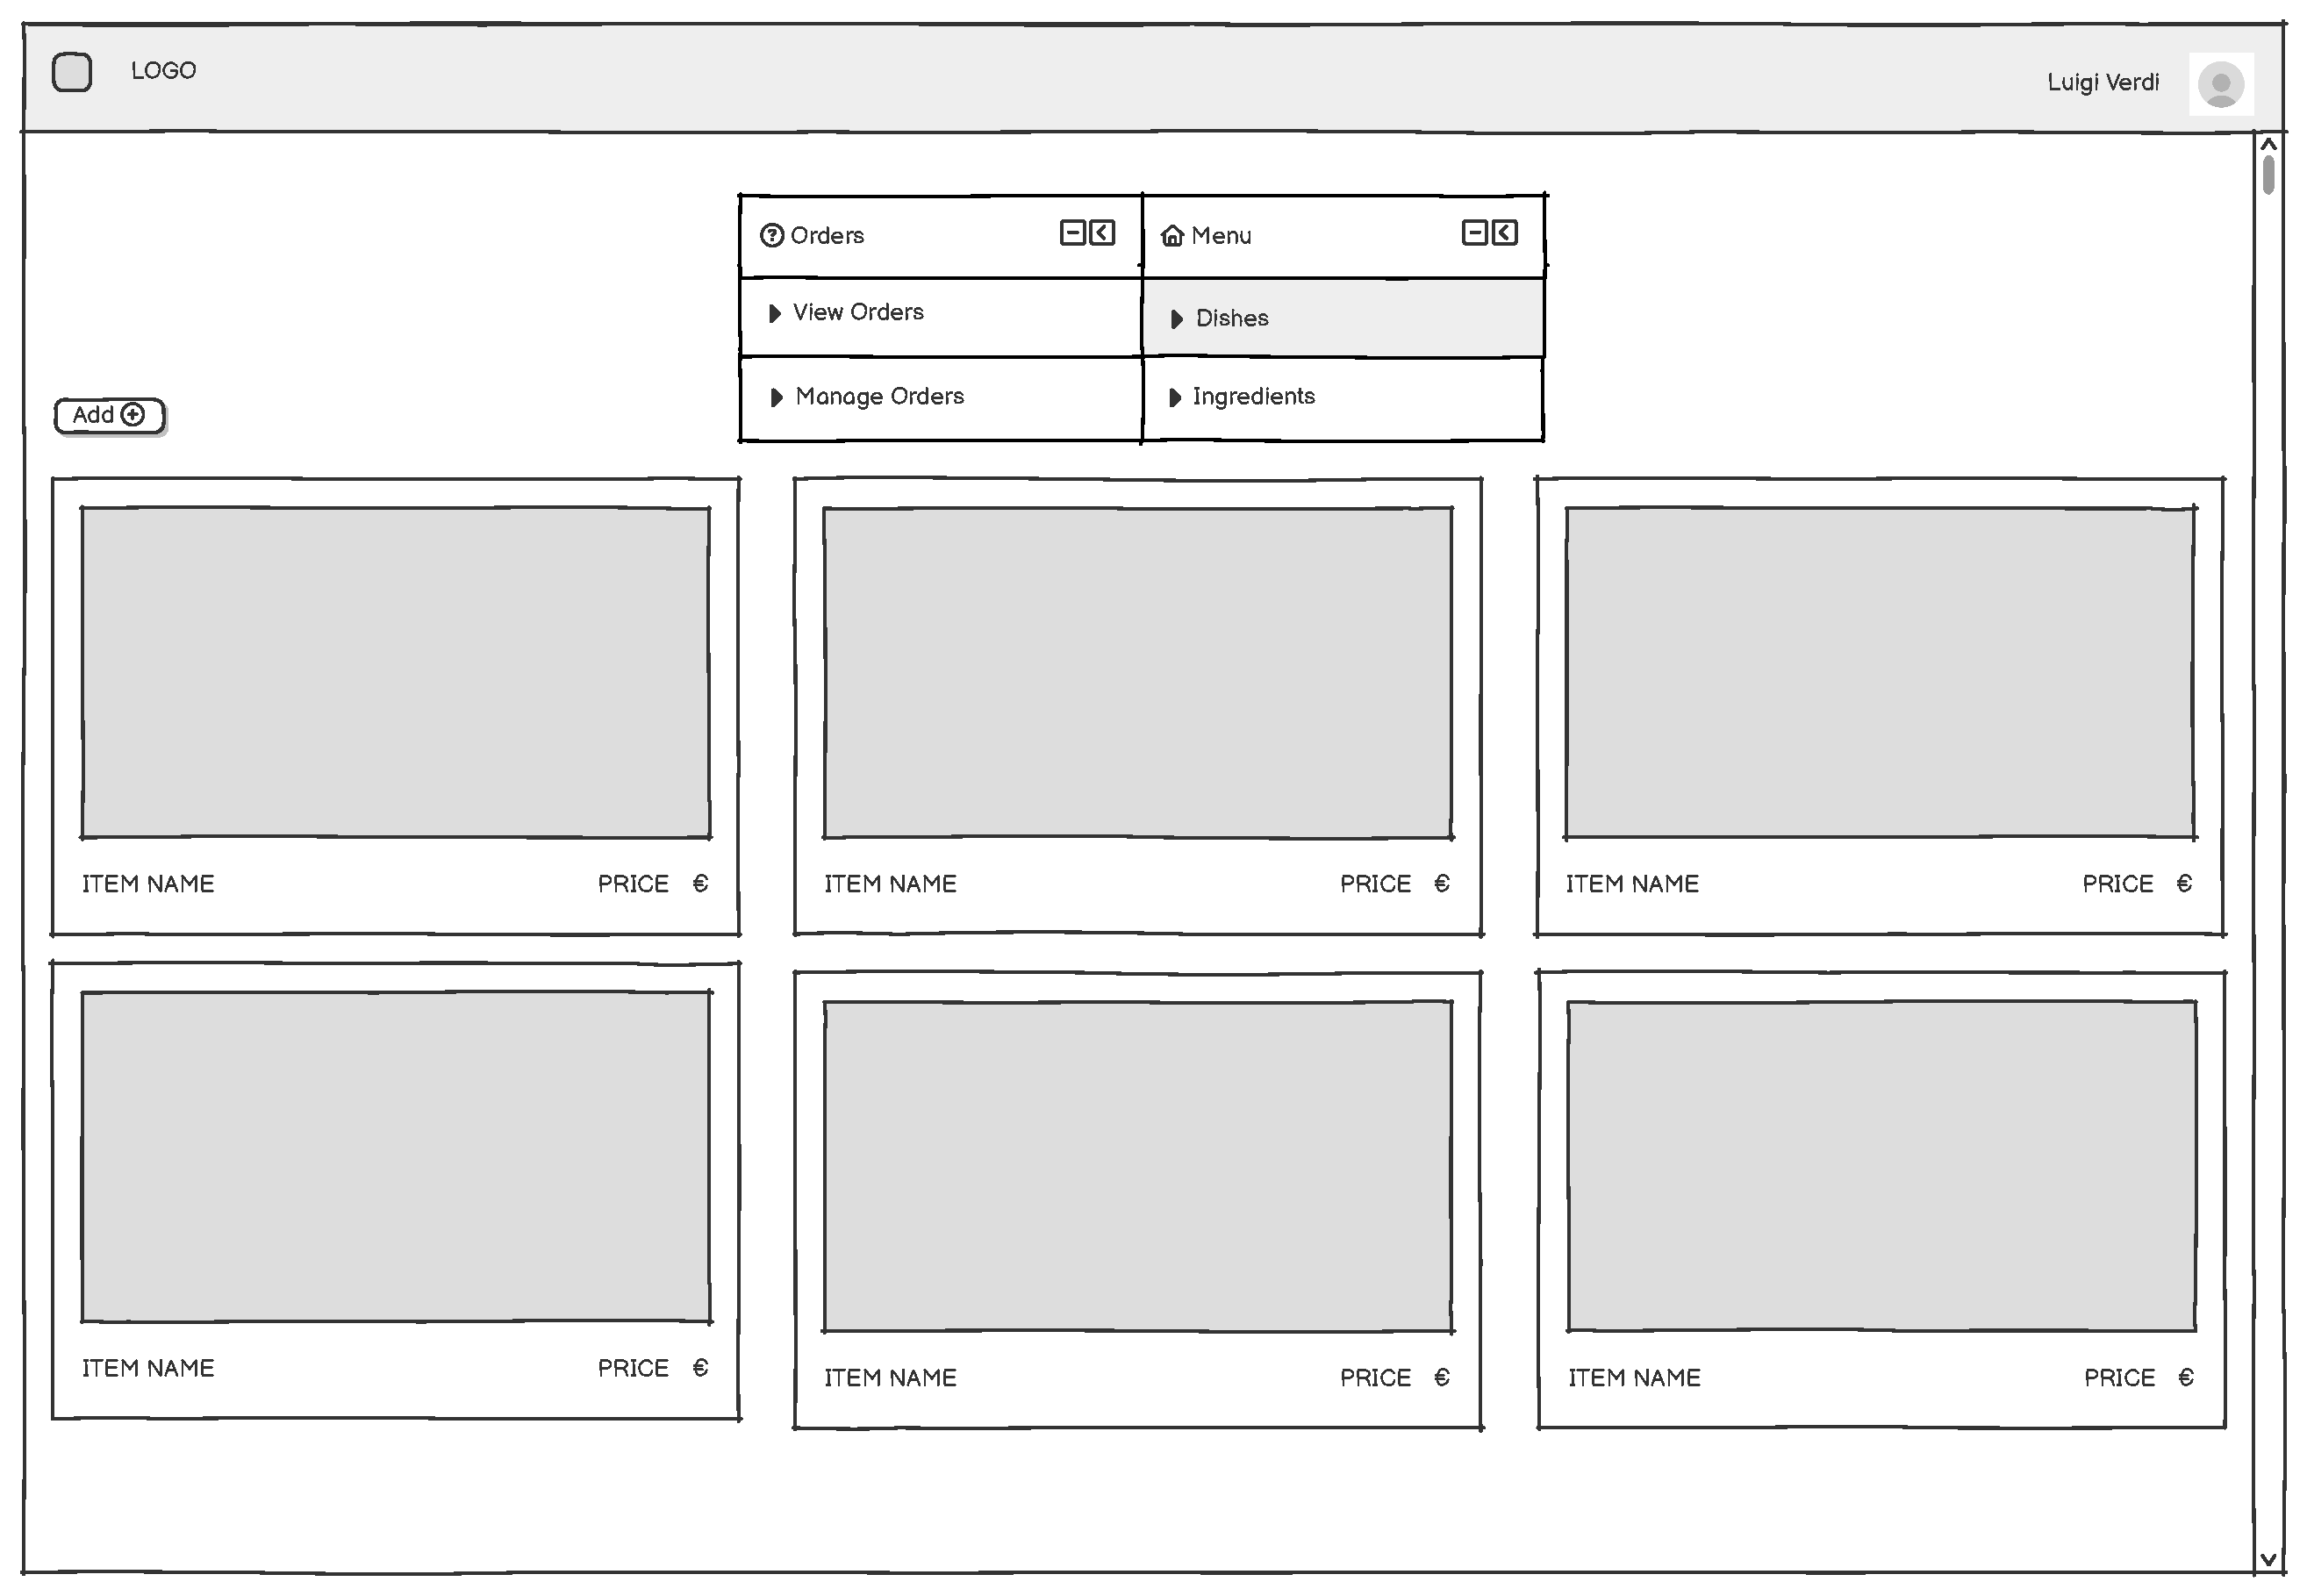
\includegraphics[width=0.8\textwidth]{images/Mockup/staffDishesList.pdf}
    \caption{Management staff-side dishes dashboard mockup page.}
    \label{fig:Management staff-side dishes dashboard mockup page.}
\end{figure}

\begin{figure}[H]
    \centering
    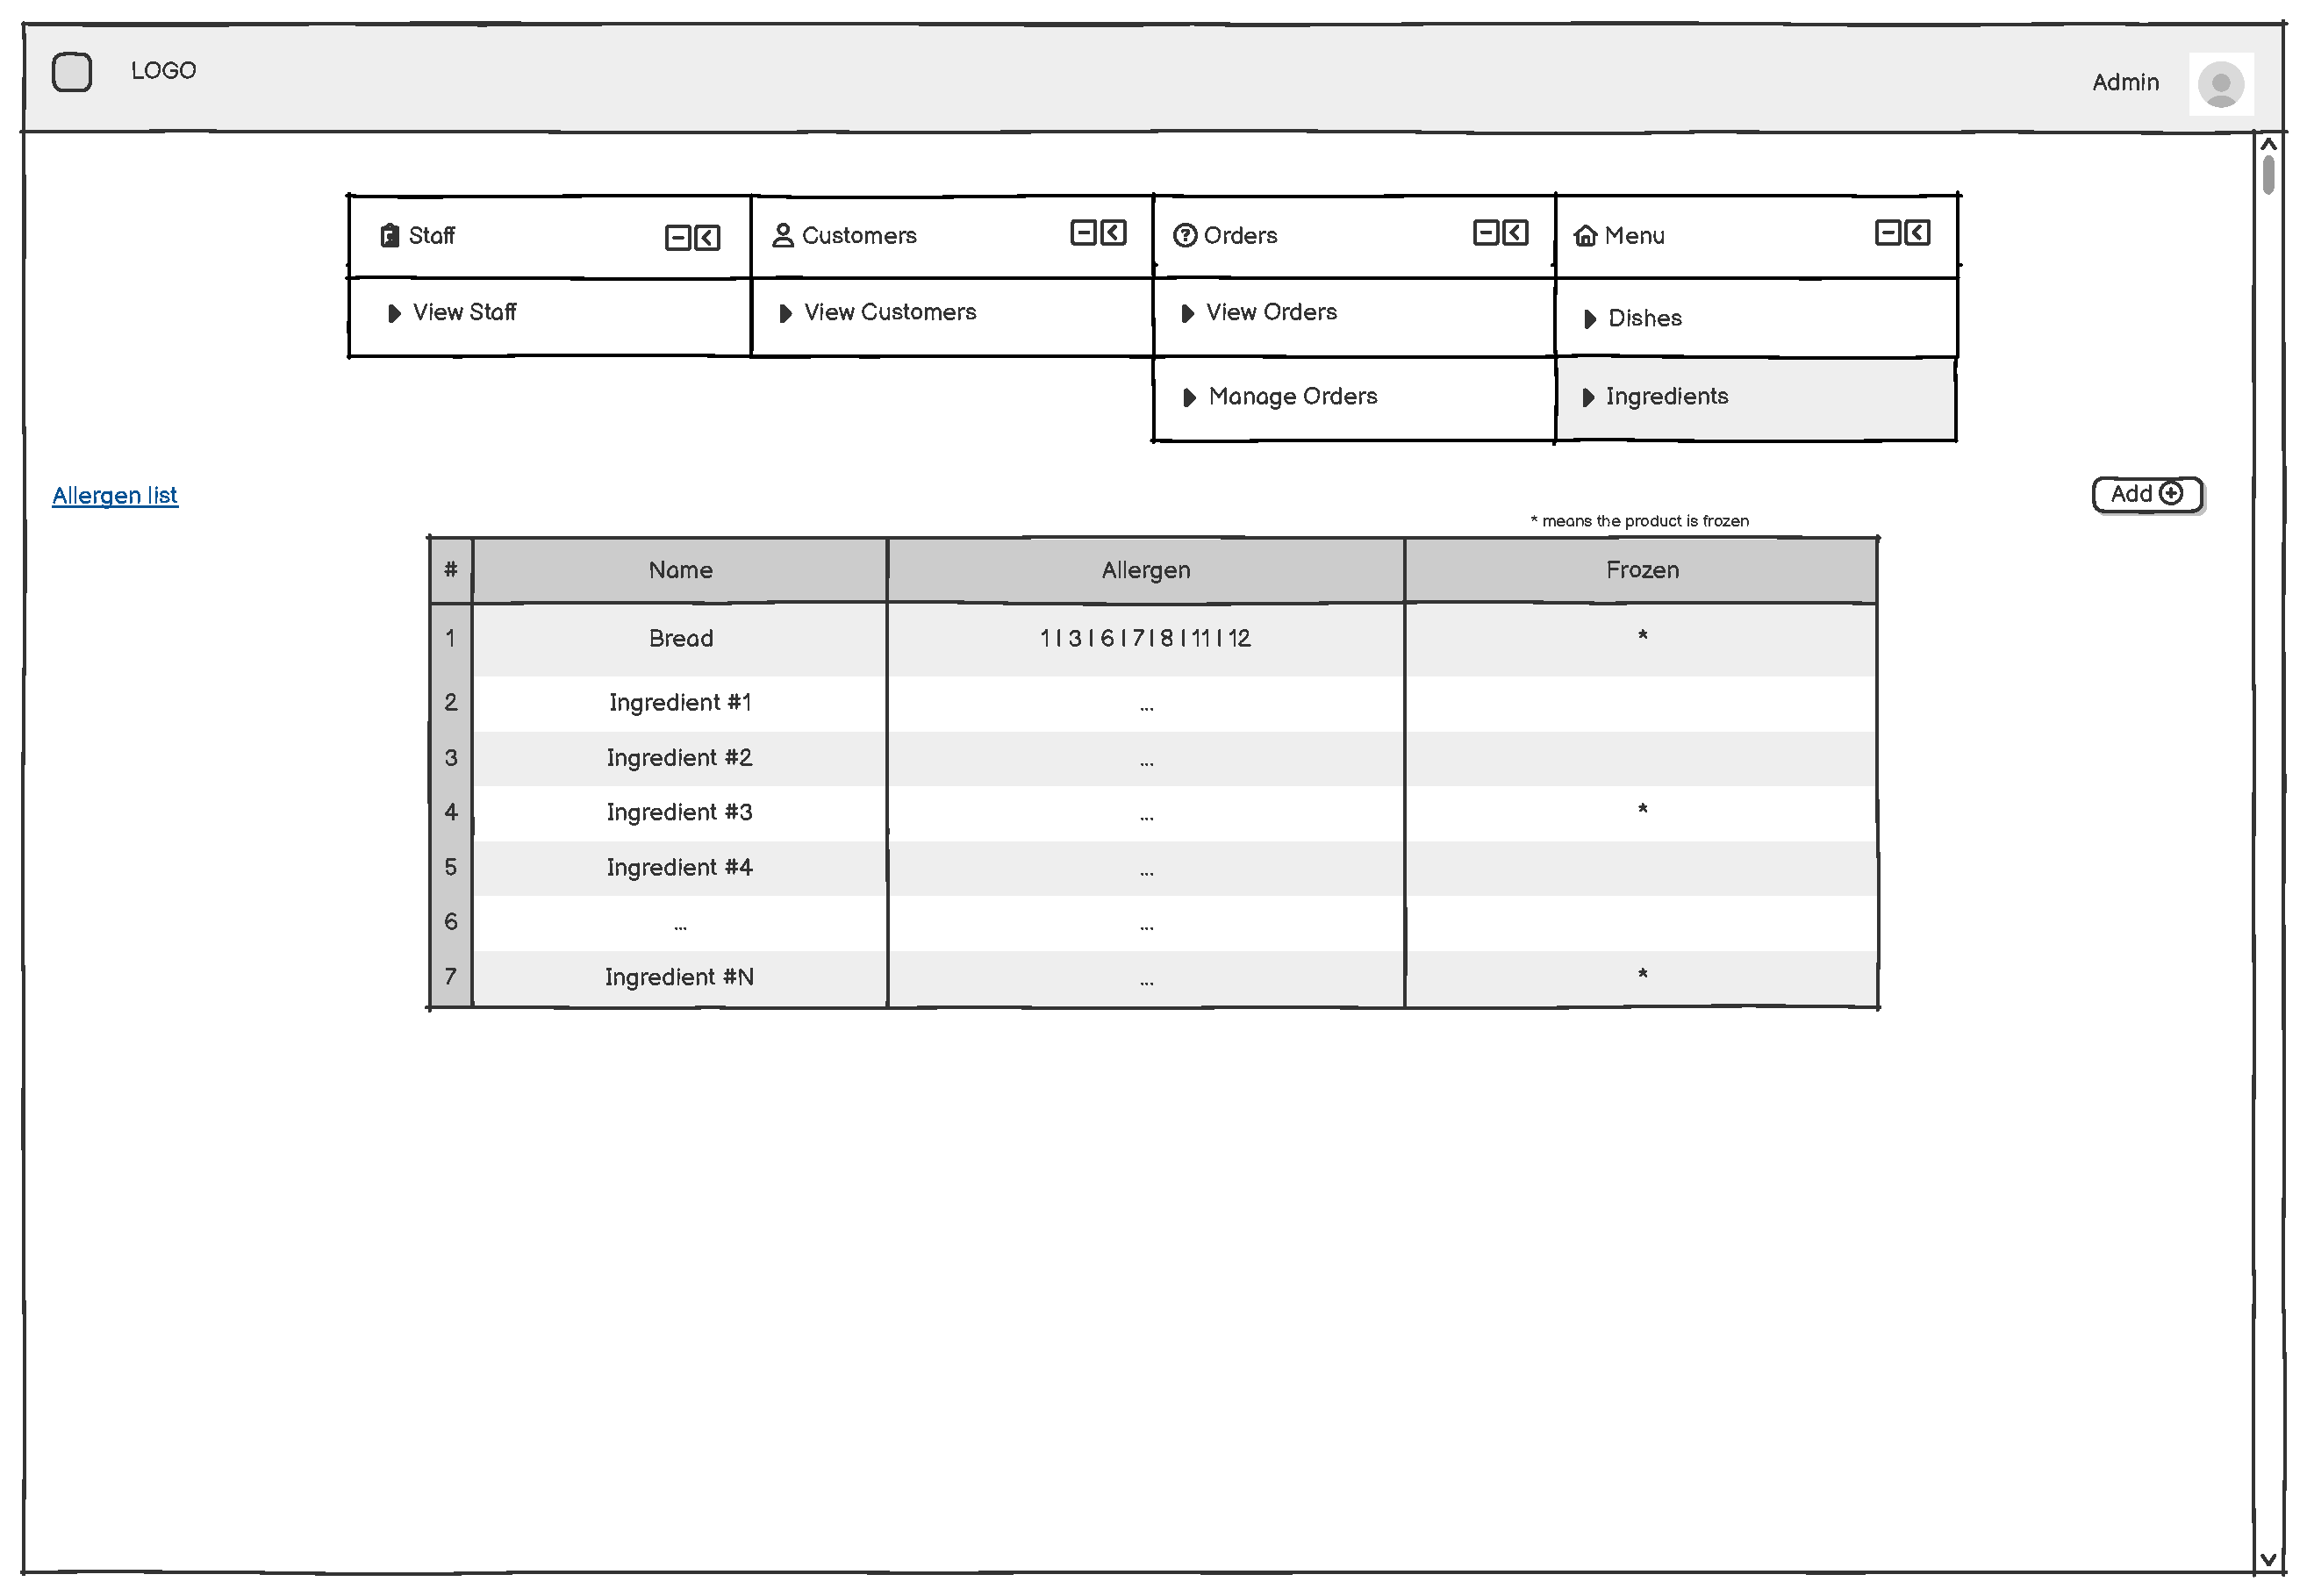
\includegraphics[width=0.8\textwidth]{images/Mockup/adminIngredients.pdf}
    \caption{Dish's ingredients admin-side mockup page.}
    \label{fig:Dish's ingredients admin-side mockup page.}
\end{figure}

\begin{figure}[H]
    \centering
    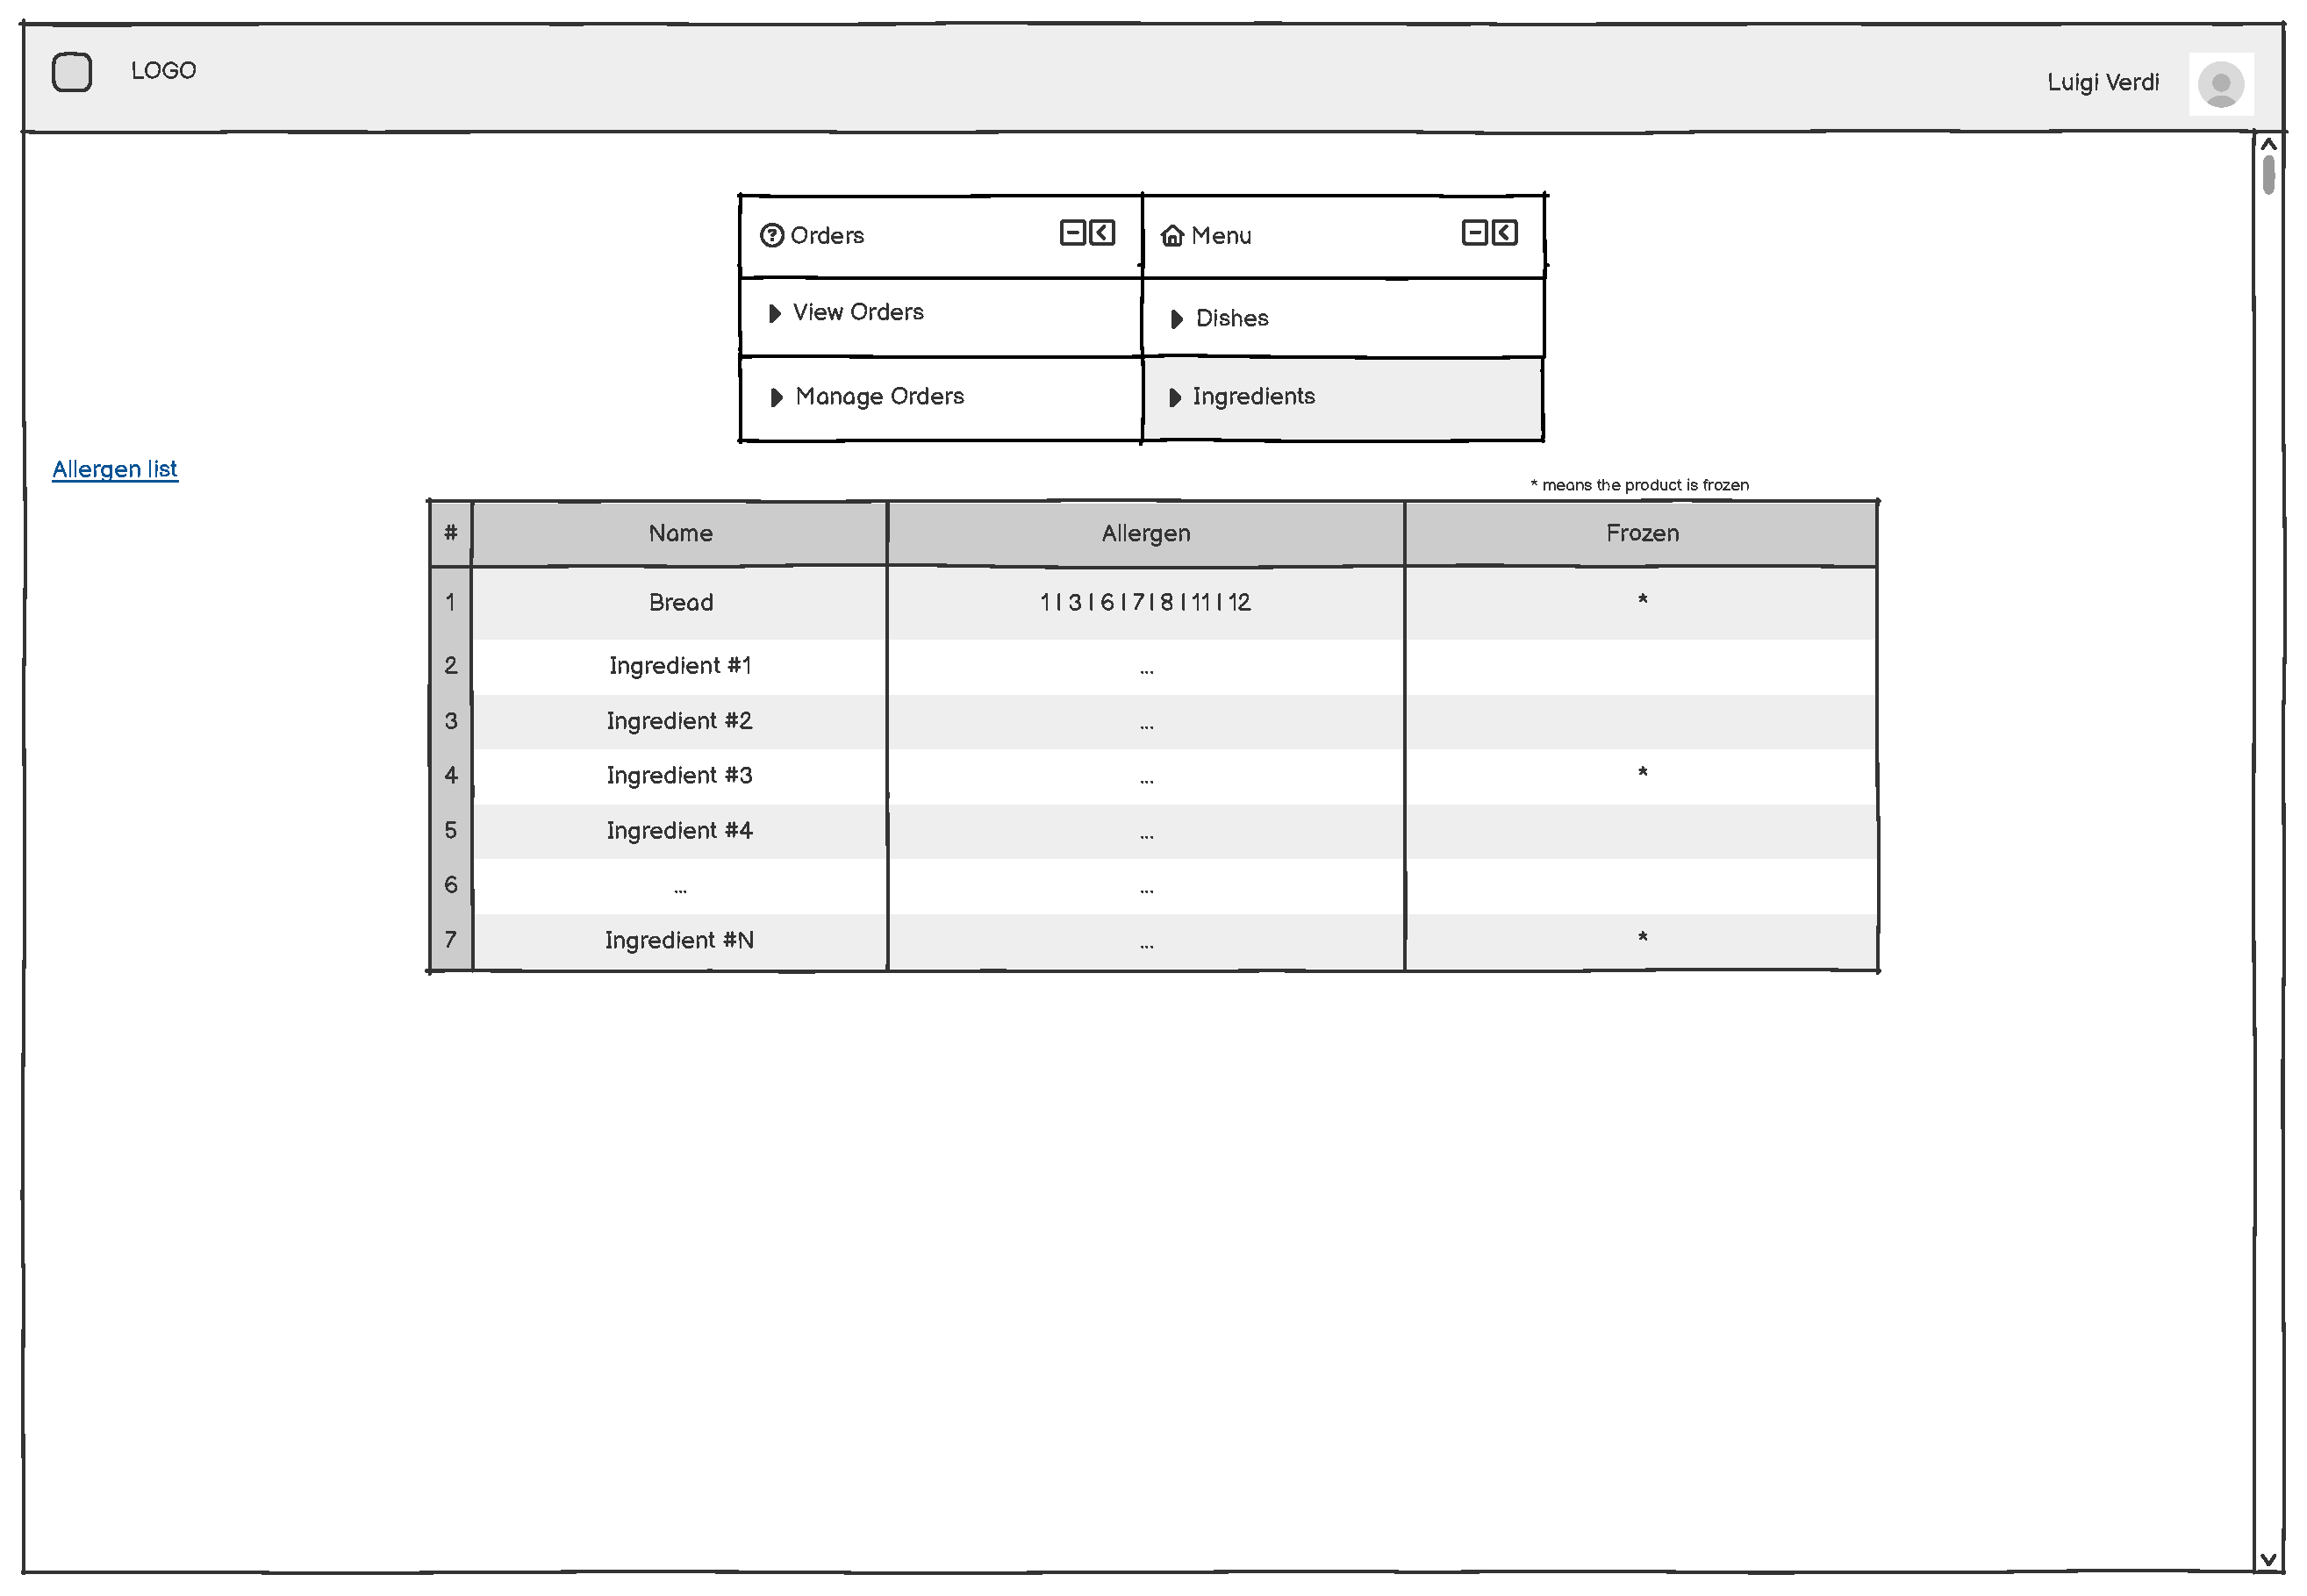
\includegraphics[width=0.8\textwidth]{images/Mockup/staffIngredients.pdf}
    \caption{Dish's ingredients staff-side mockup page.}
    \label{fig:Dish's ingredients staff-side mockup page.}
\end{figure}

\begin{figure}[H]
    \centering
    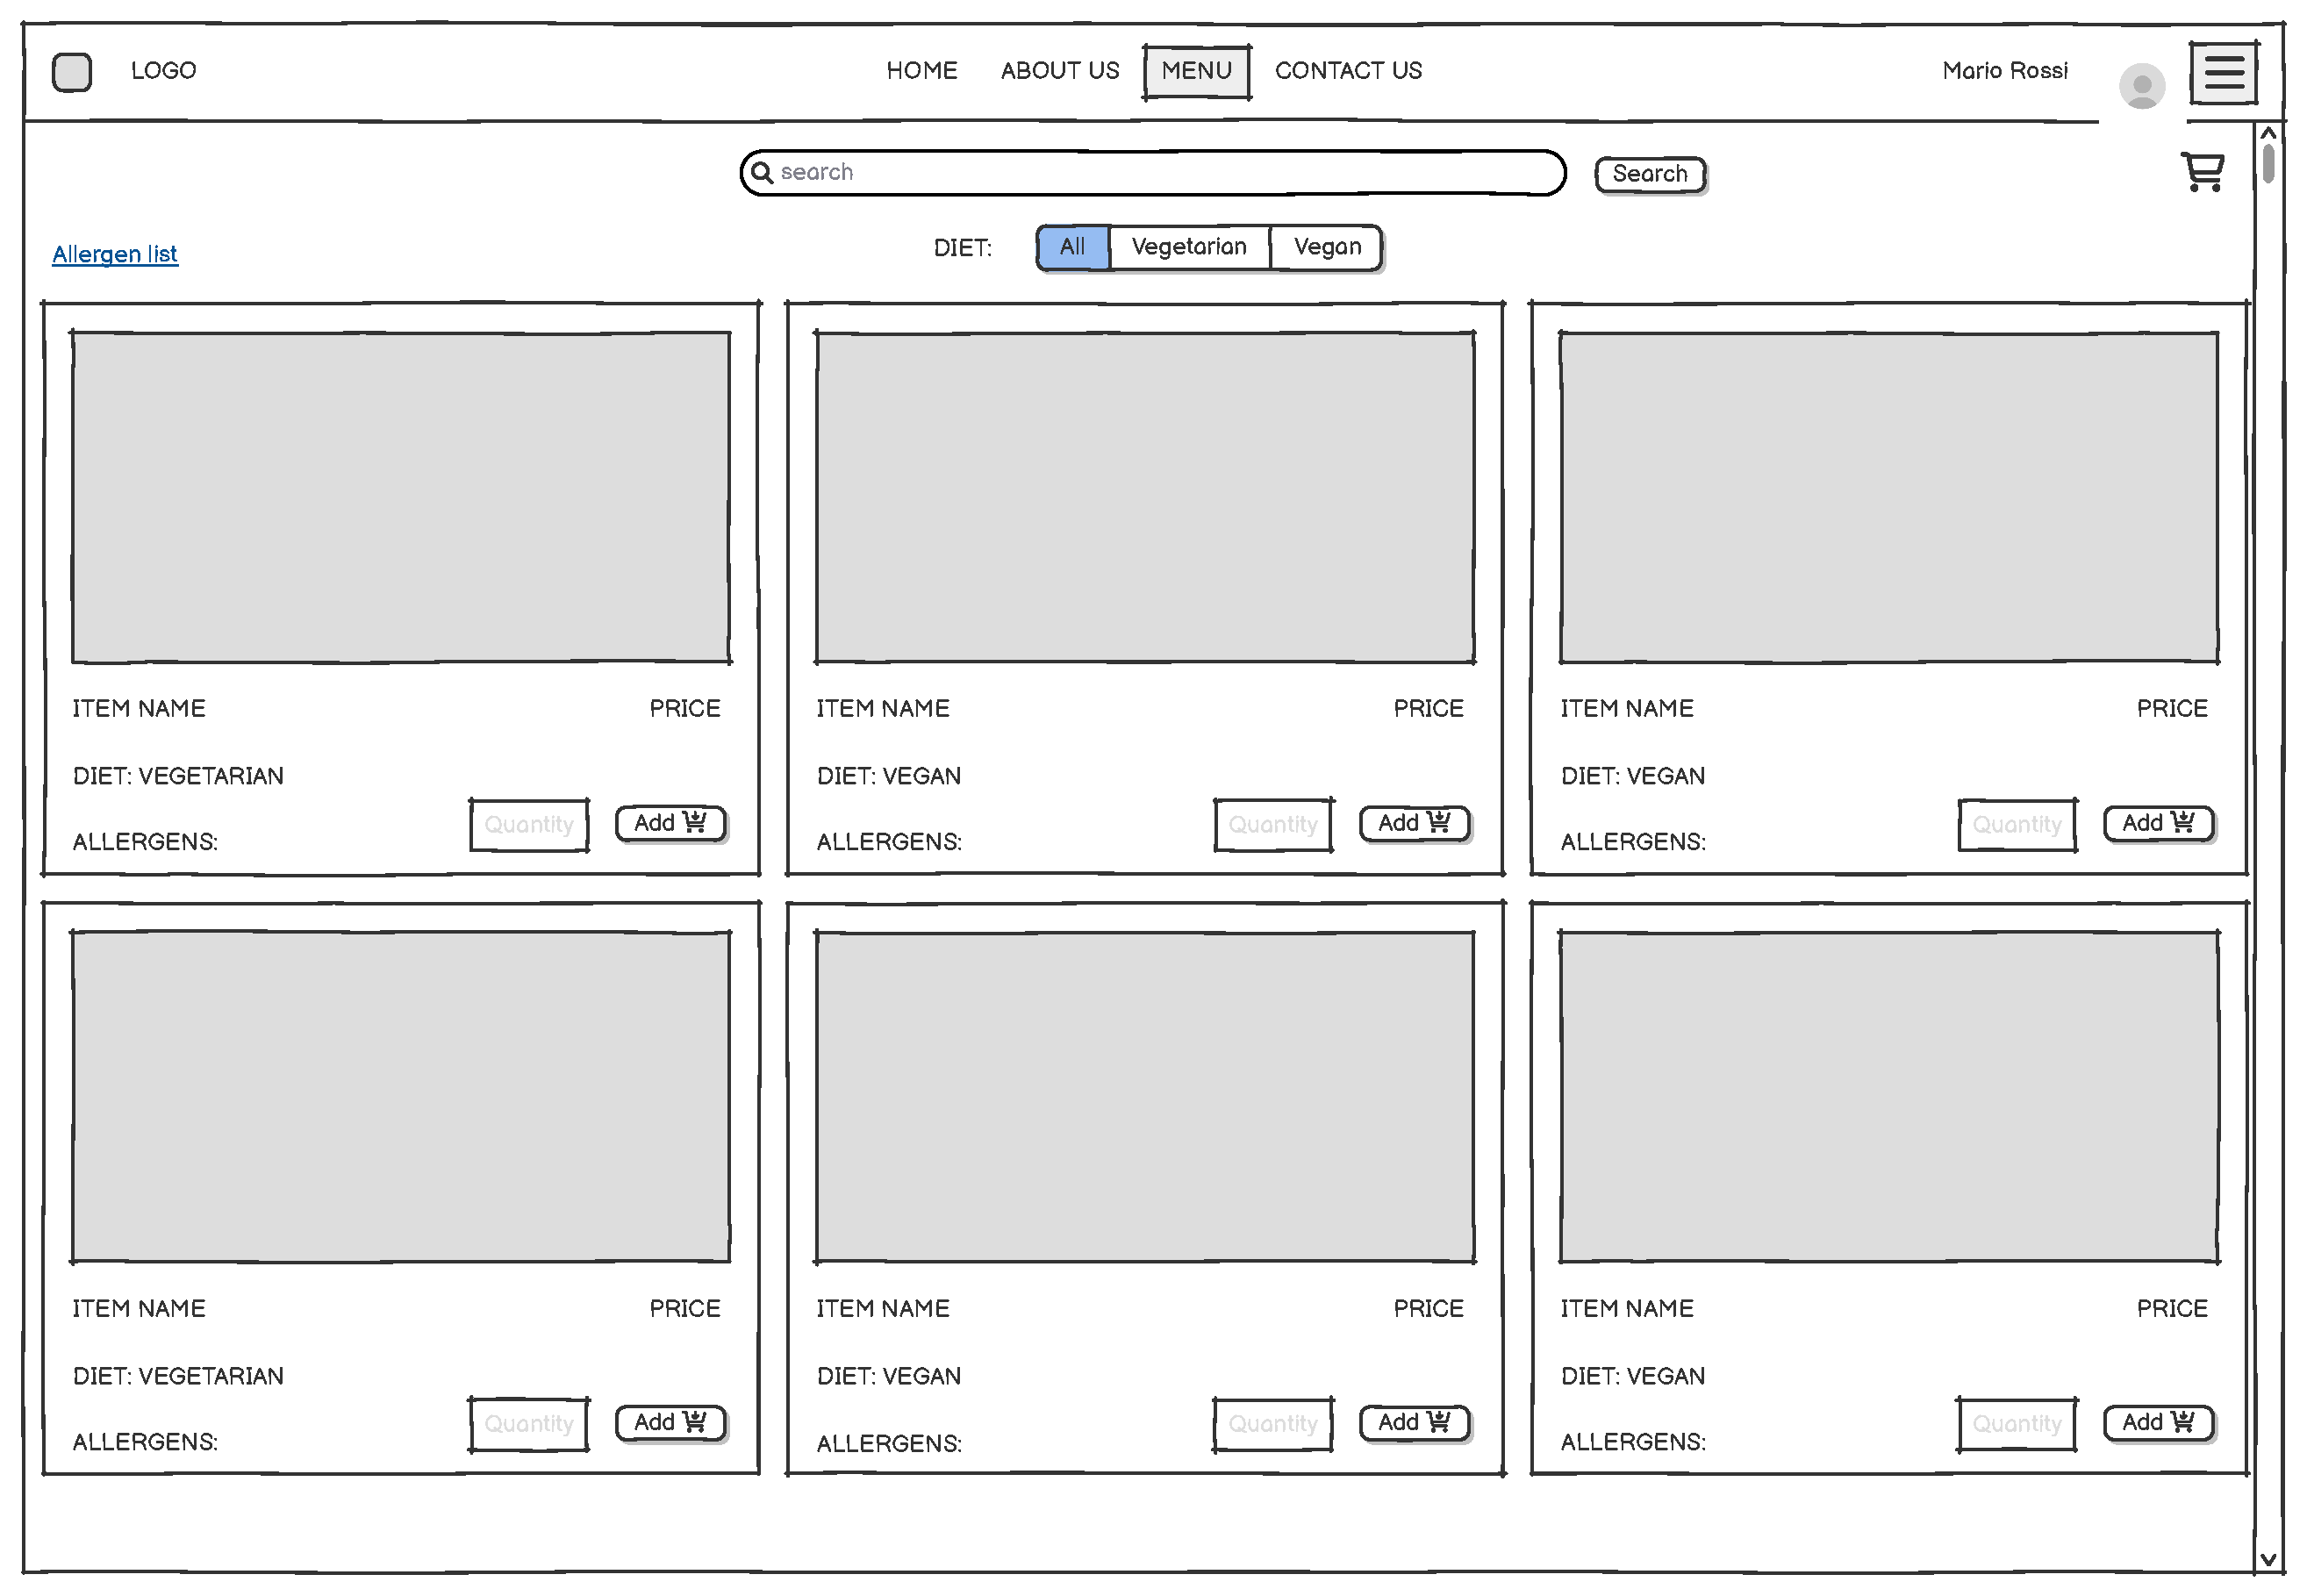
\includegraphics[width=0.8\textwidth]{images/Mockup/menu.pdf}
    \caption{Menu dashboard's mockup page.}
    \label{fig:Menu dashboard's mockup page.}
\end{figure}

\subsection{Other mockups}

The following mockups complete the presentation layer by showing the secondary pages used by customers, staff members and administrators. They focus on cart handling, order tracking, account management and the back-office tools needed to supervise users and orders.

\begin{figure}[H]
    \centering
    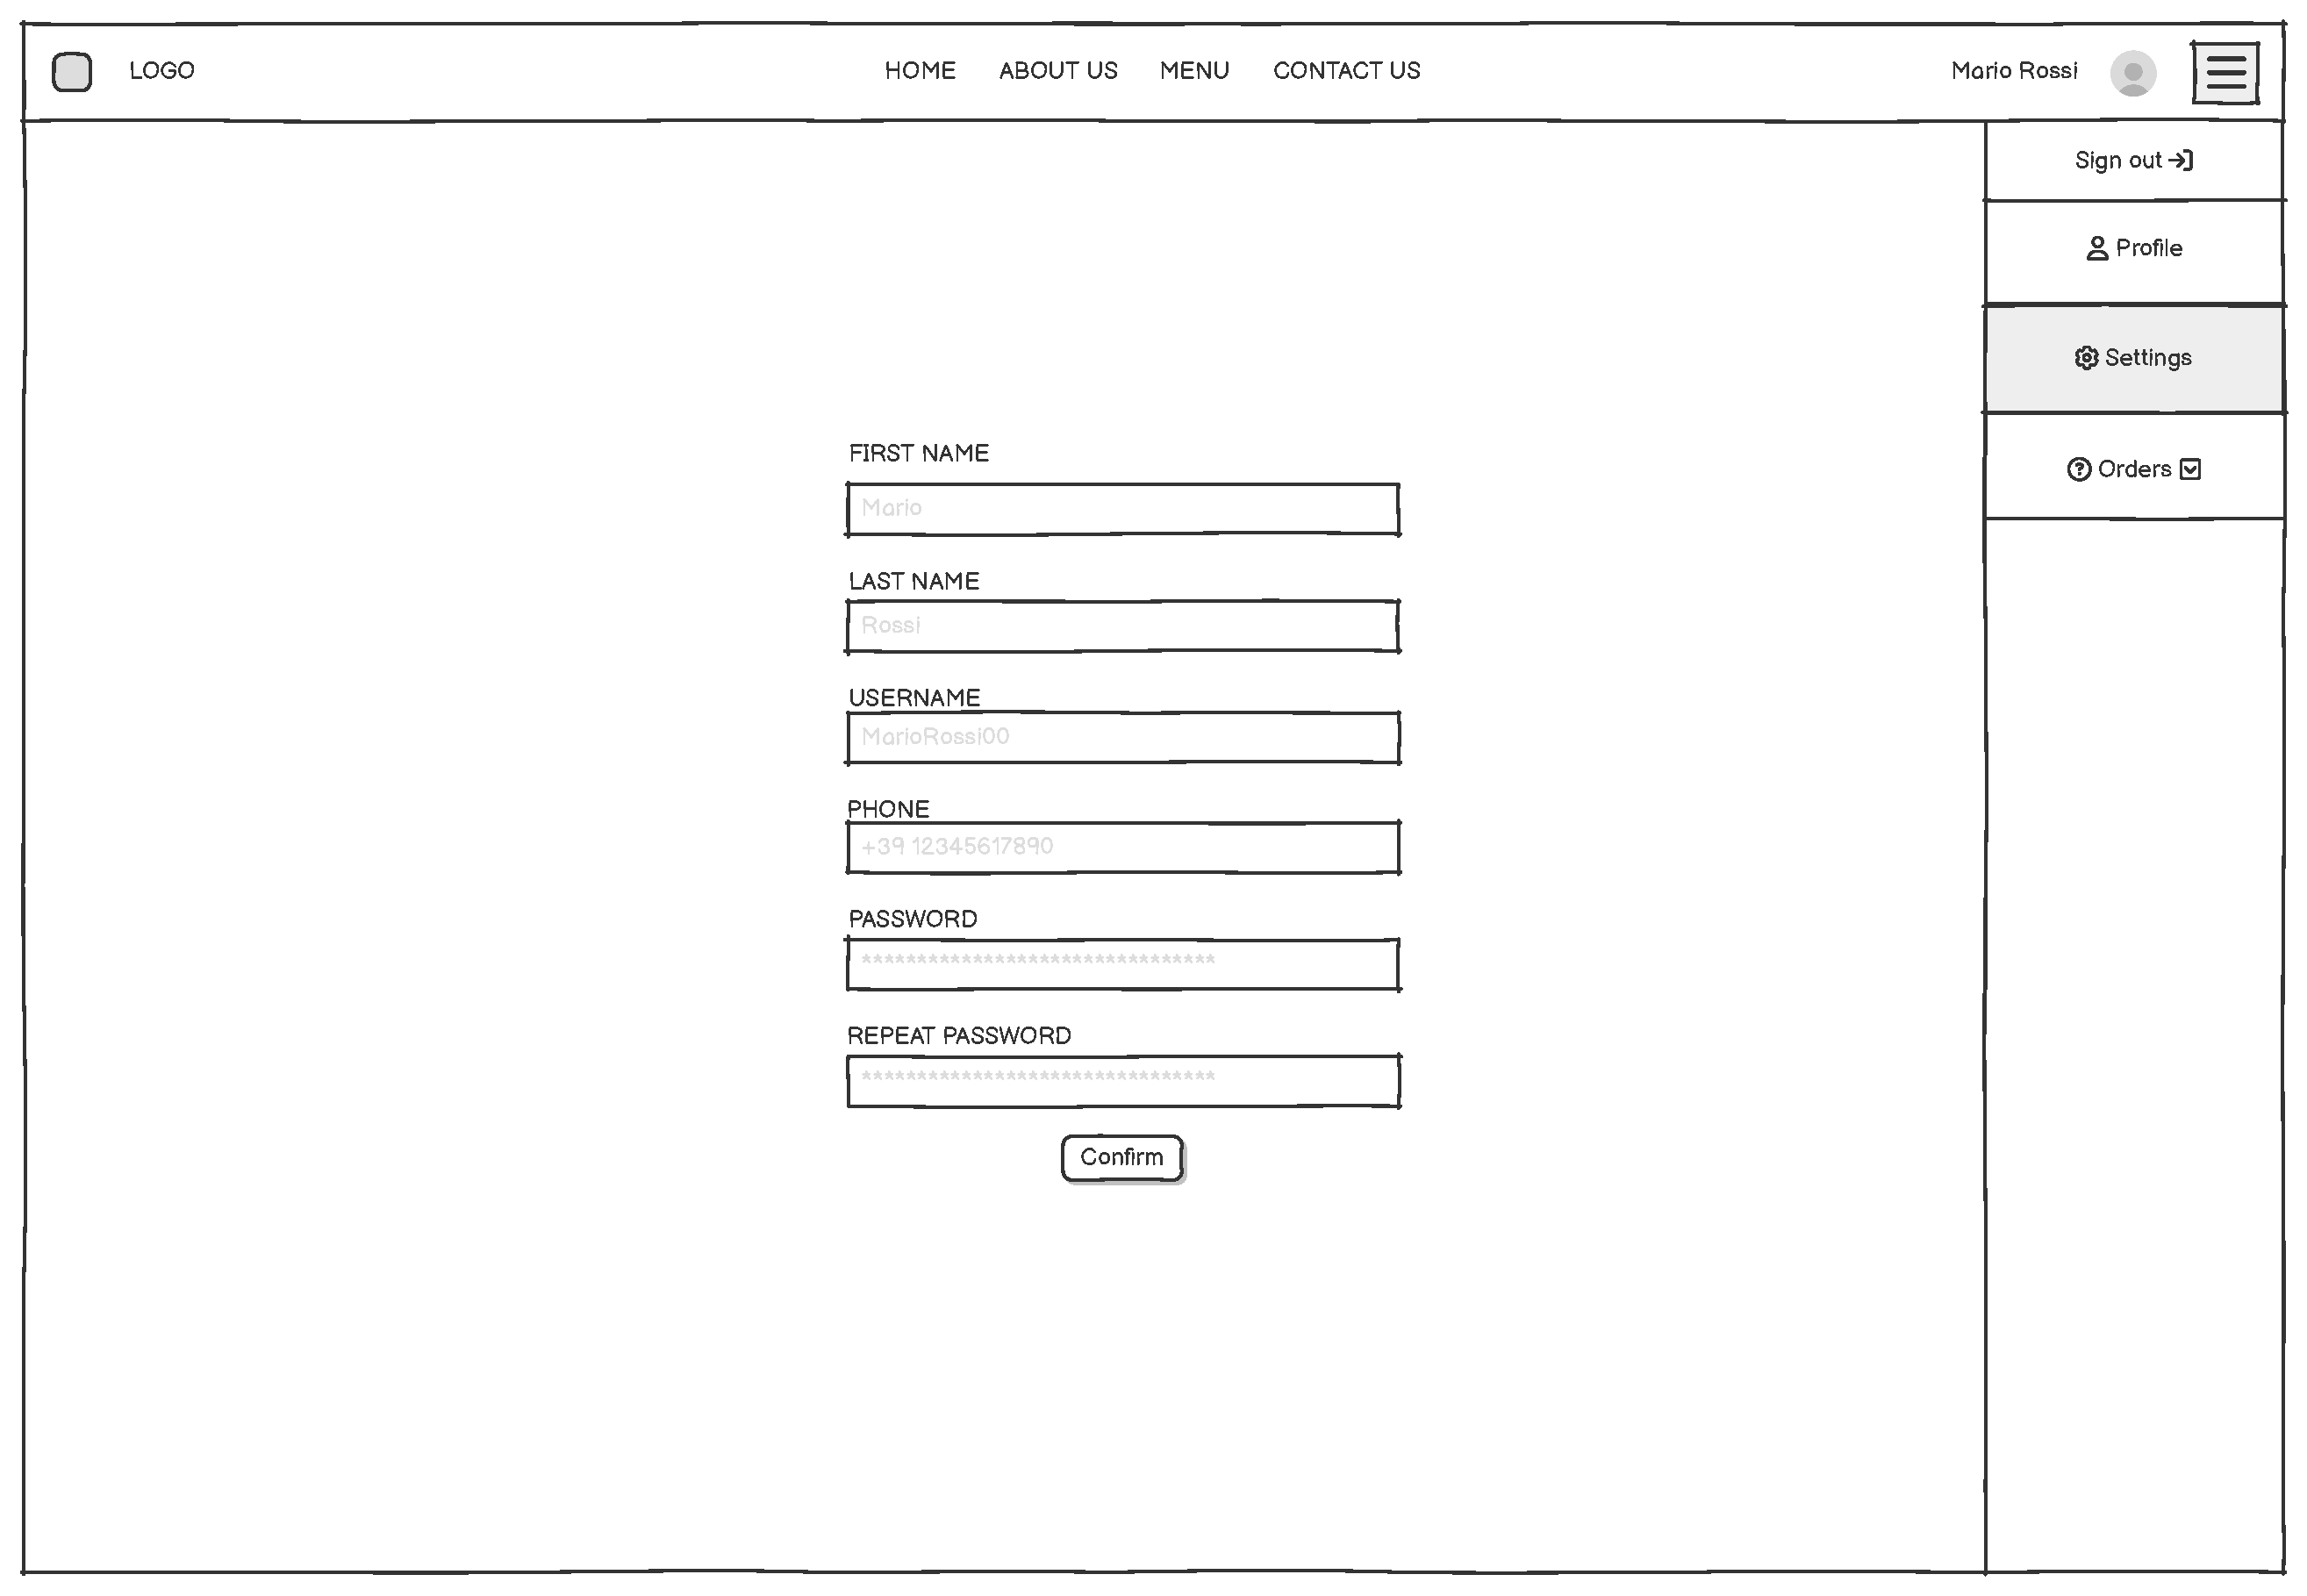
\includegraphics[width=0.55\textwidth]{images/Mockup/profileSettings.pdf}
    \caption{Profile's mockup page. The profile settings page allows users to consult and update their personal account information. It keeps account-related actions separated from the ordering flow while remaining accessible from the authenticated area.}
    \label{fig:Profile's page section.}
\end{figure}

\begin{figure}[H]
    \centering
    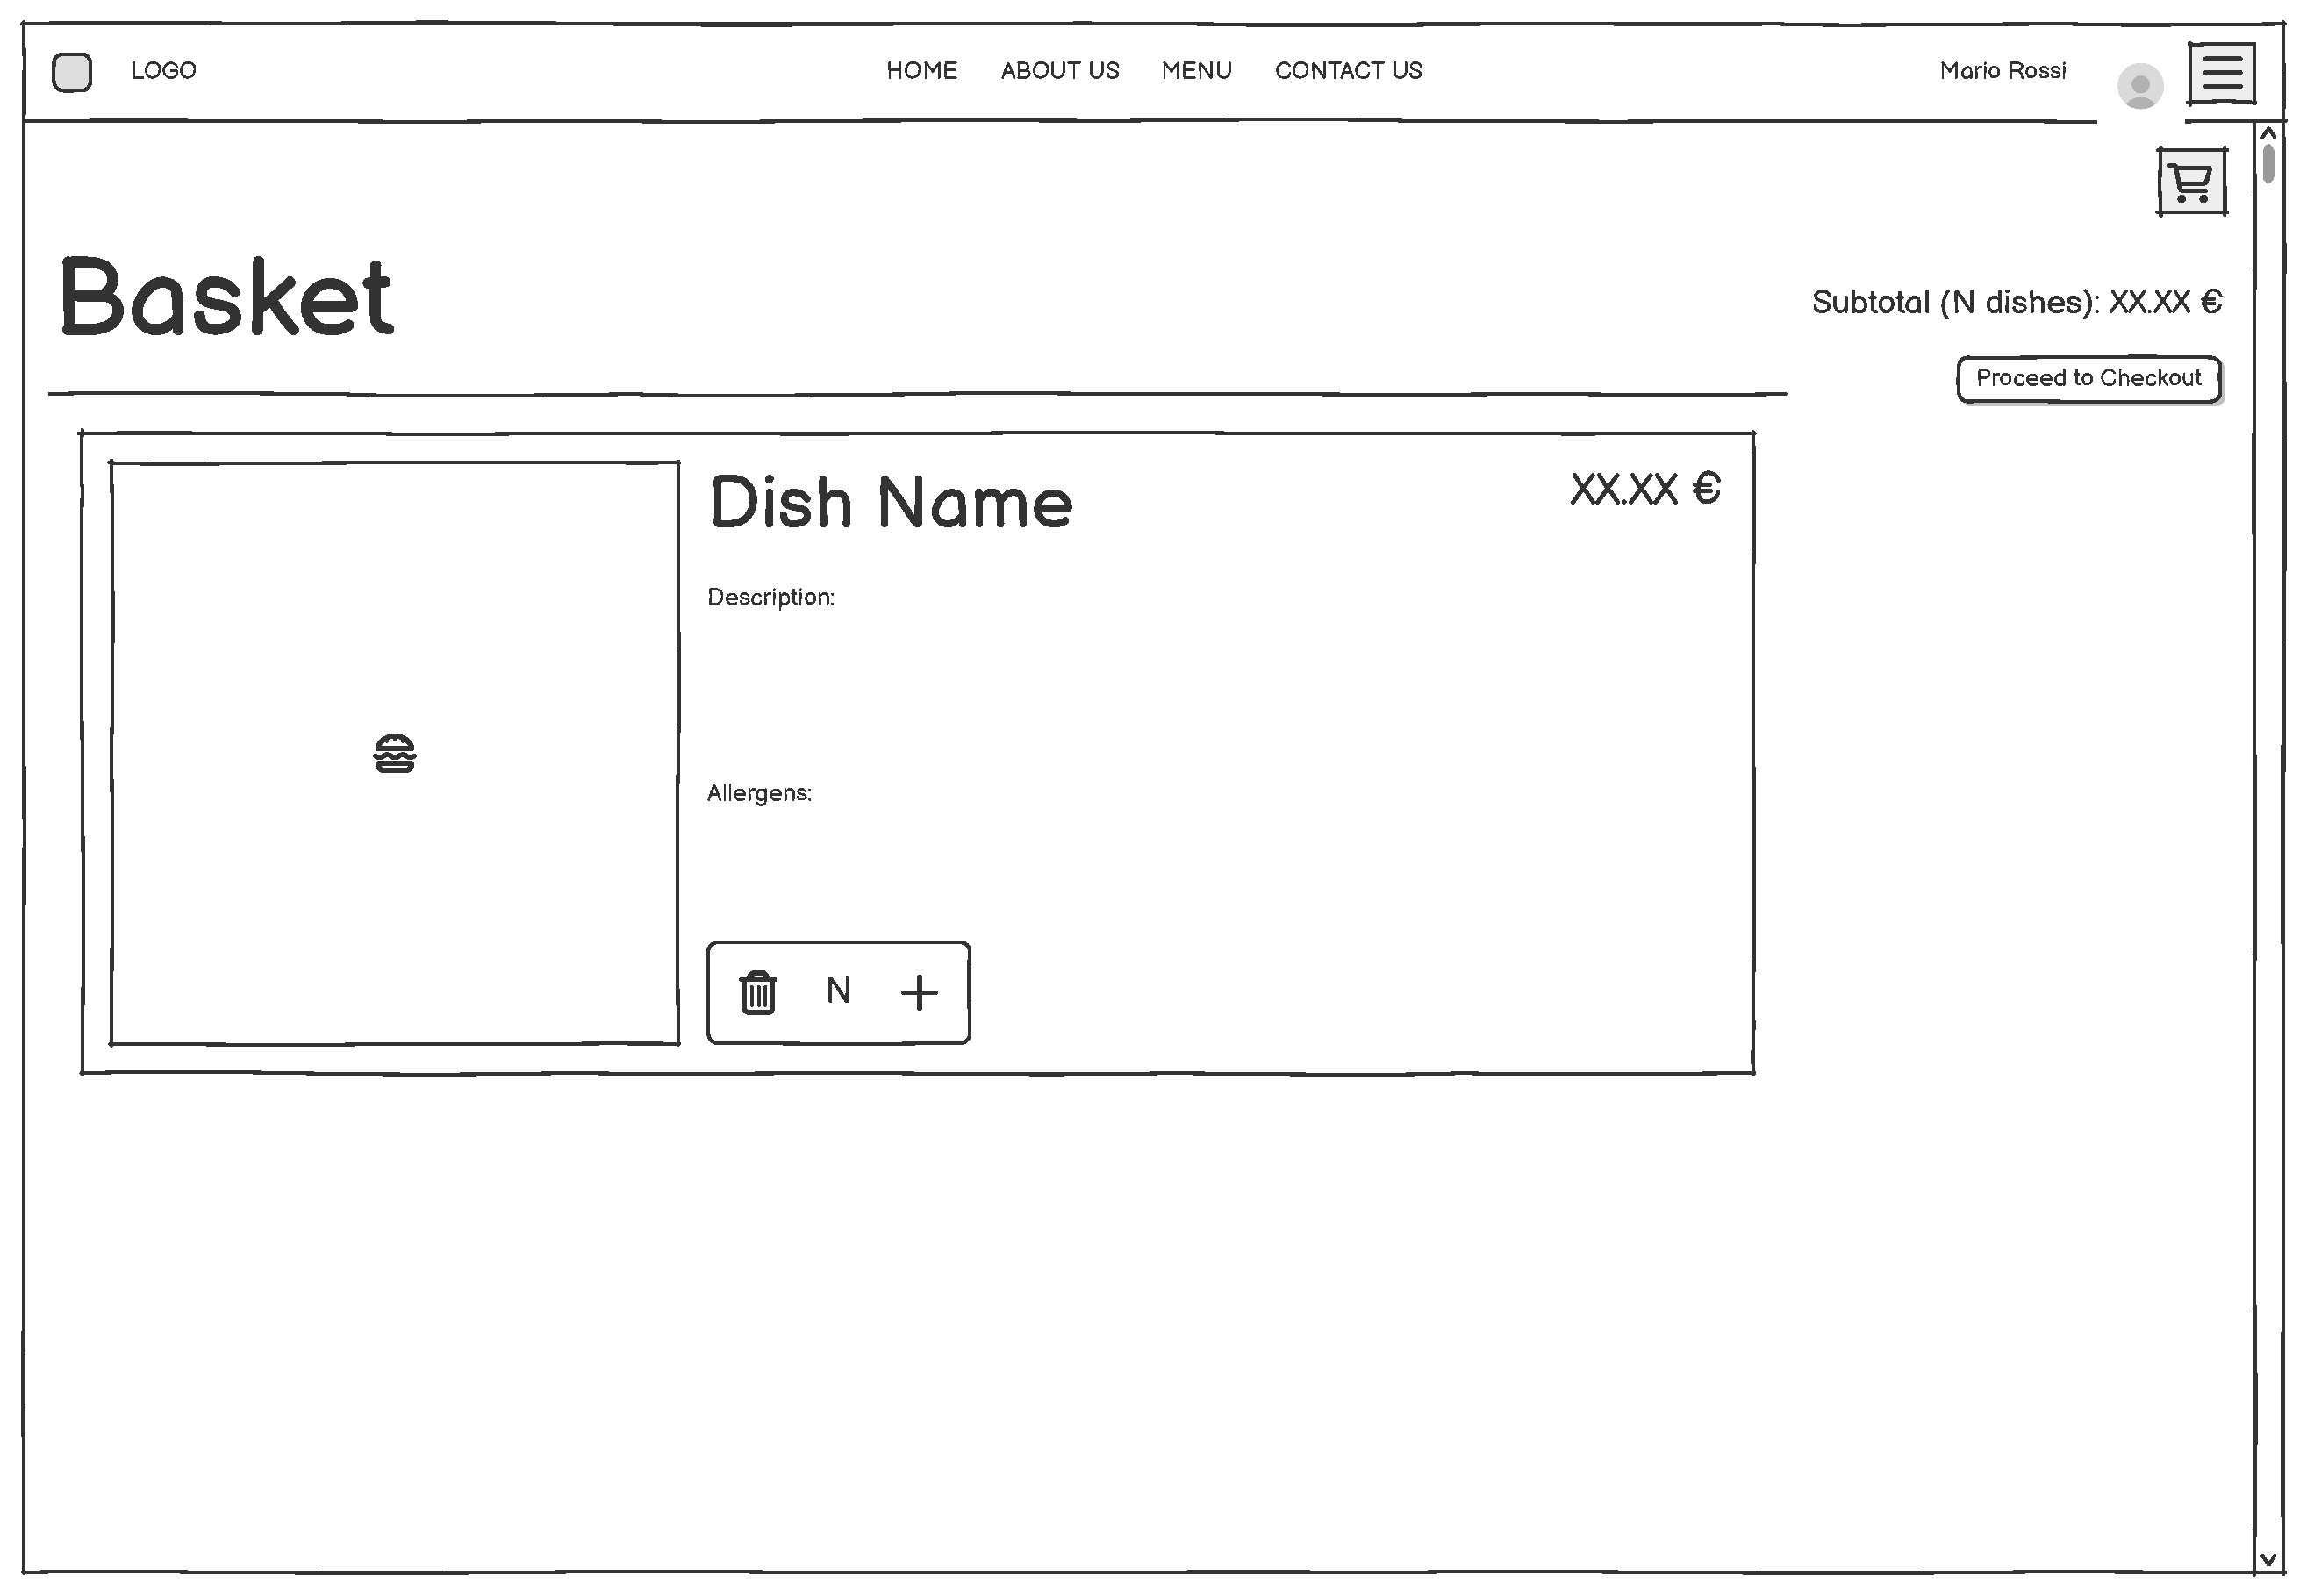
\includegraphics[width=0.55\textwidth]{images/Mockup/carrello.pdf}
    \caption{Shopping cart mockup page. The shopping cart page lets customers review the dishes selected from the menu before submitting an order. It provides a compact summary of the chosen items, quantities, and total amount, allowing the user to adjust the order before confirmation.}
    \label{fig:Shopping cart mockup page.}
\end{figure}

\begin{figure}[htbp]
    \centering
    \caption{Orders' view custome-side mockup page.}
    % Prima immagine
    \begin{subfigure}[t]{0.47\textwidth}
        \centering
        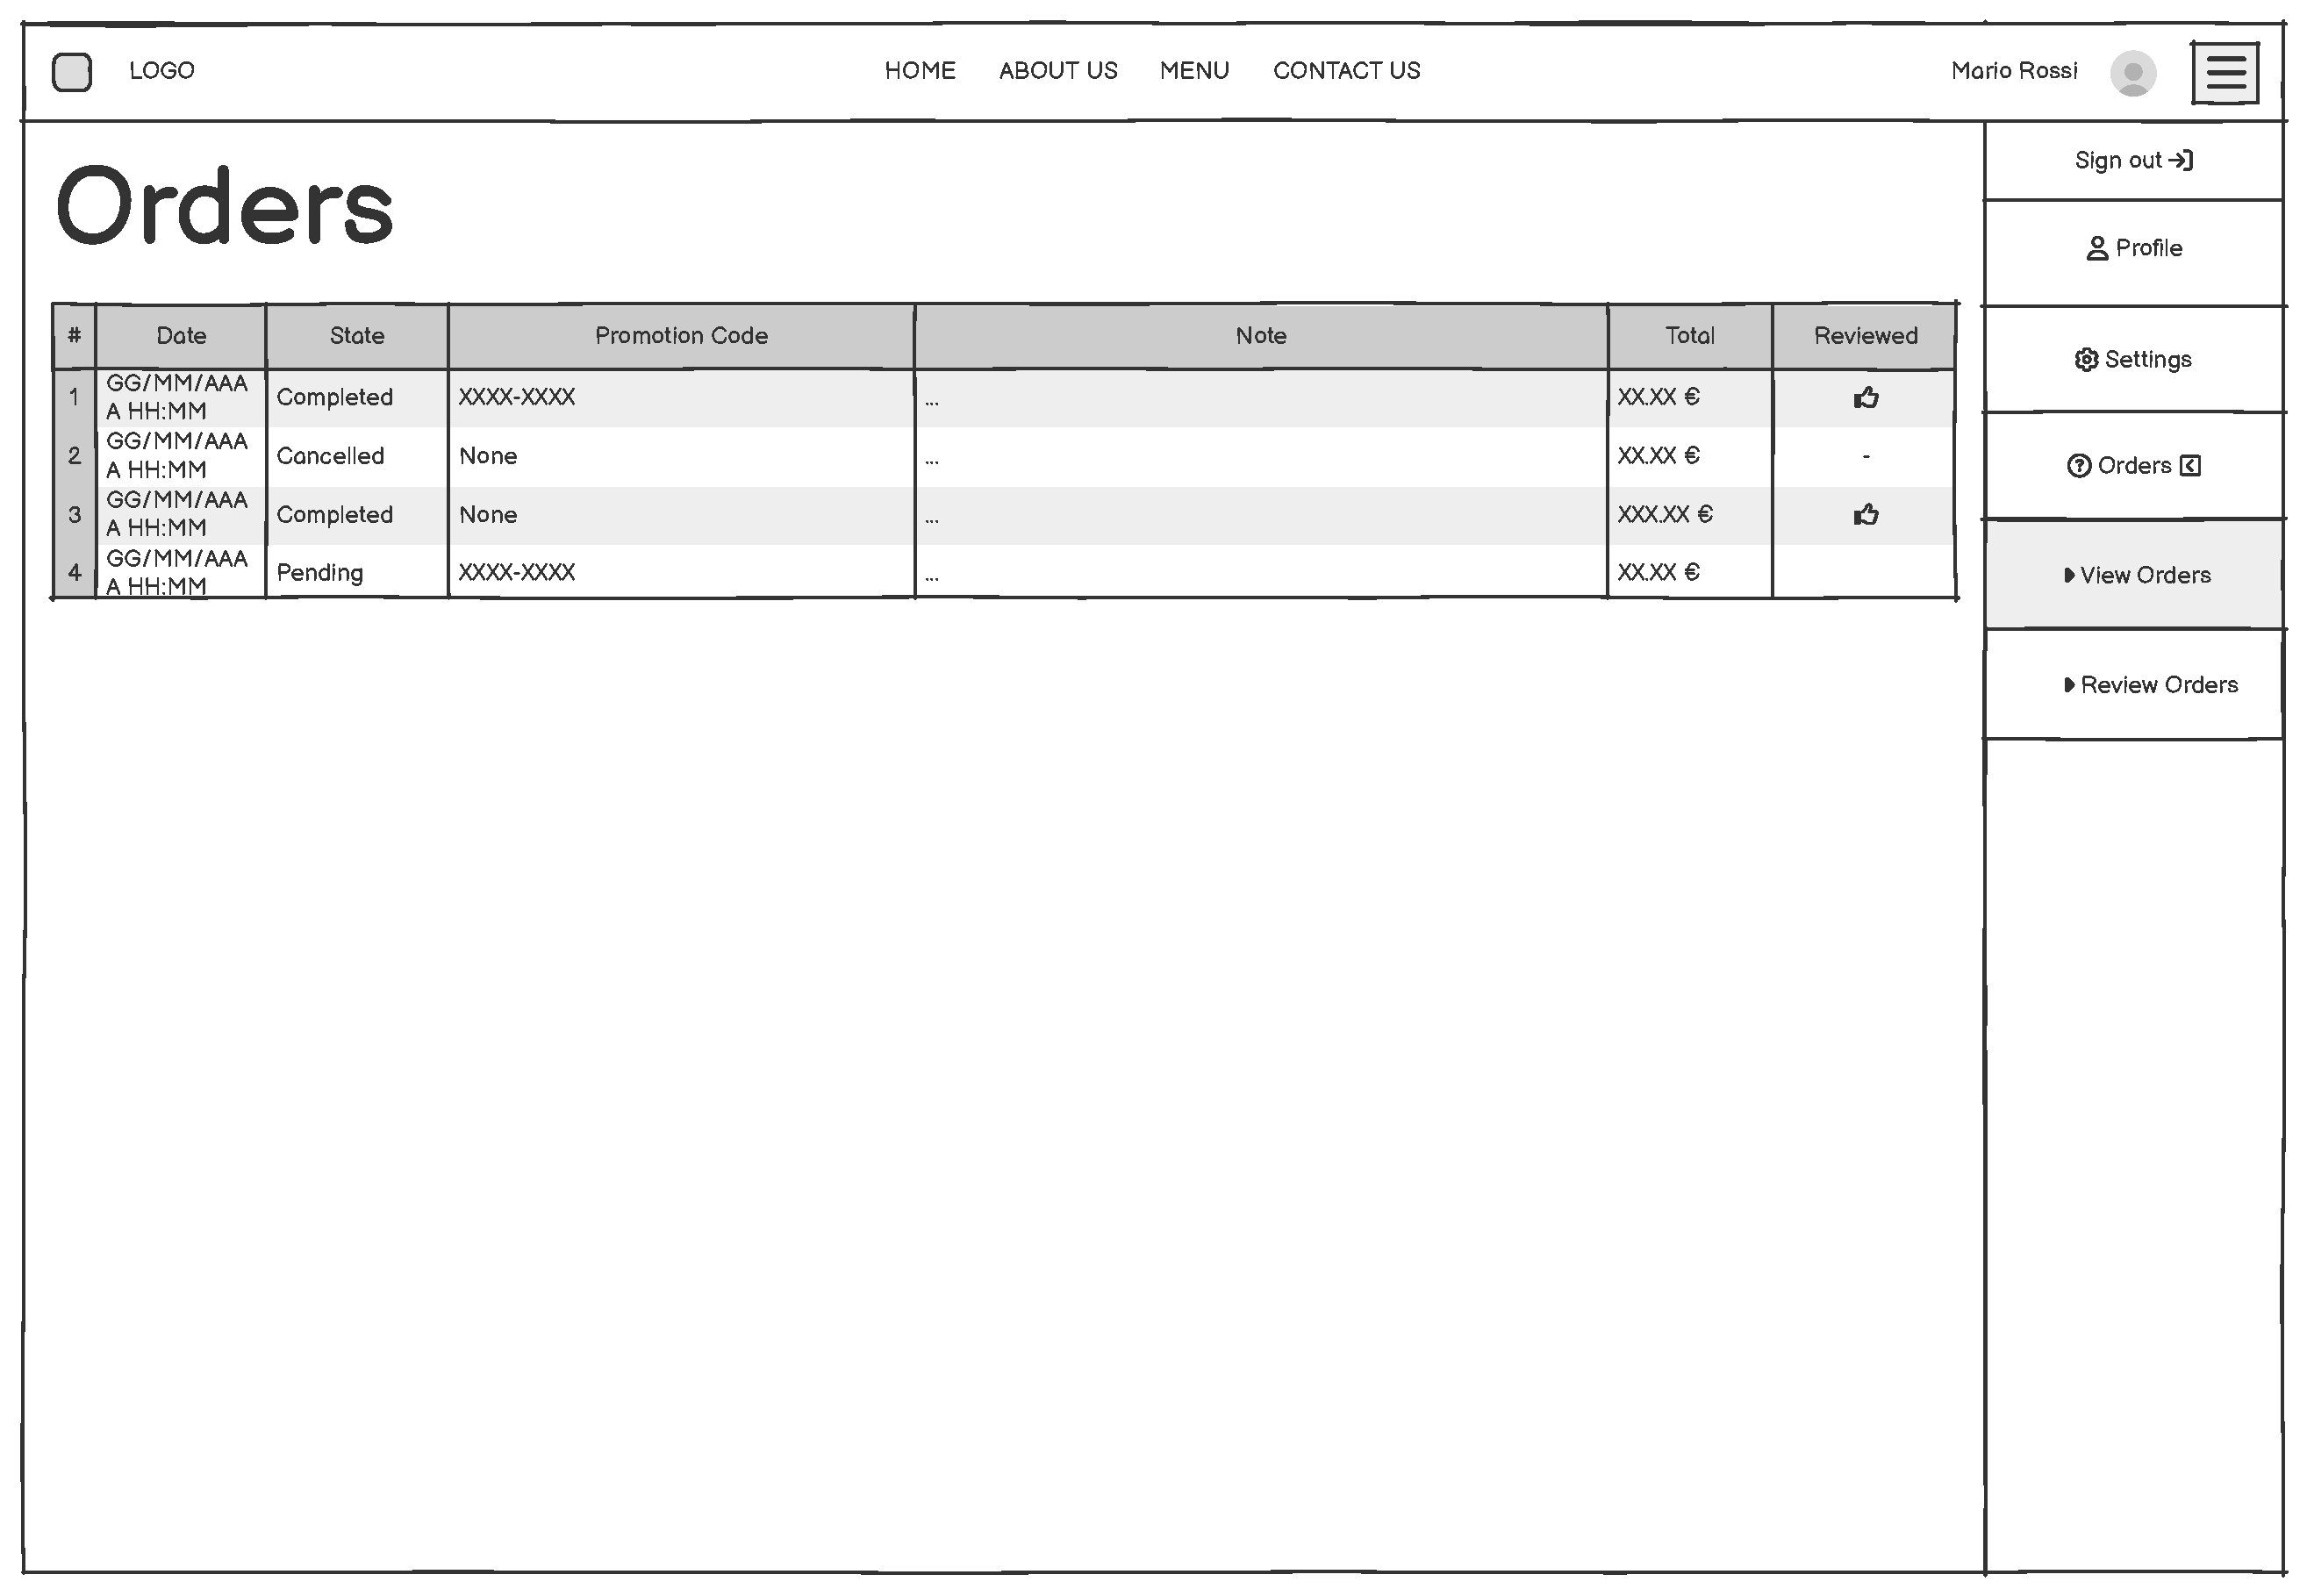
\includegraphics[width=\textwidth]{images/Mockup/orders.pdf}
        \caption{Customer's orders mockup page. The customer's orders page allows authenticated customers to monitor their own orders. It shows the relevant order information and helps users understand the current state of each request.}
        \label{fig:Customer's orders mockup page.}
    \end{subfigure}
    \hfill % Spazio orizzontale tra le immagini
    % Seconda immagine
    \begin{subfigure}[t]{0.47\textwidth}
        \centering
        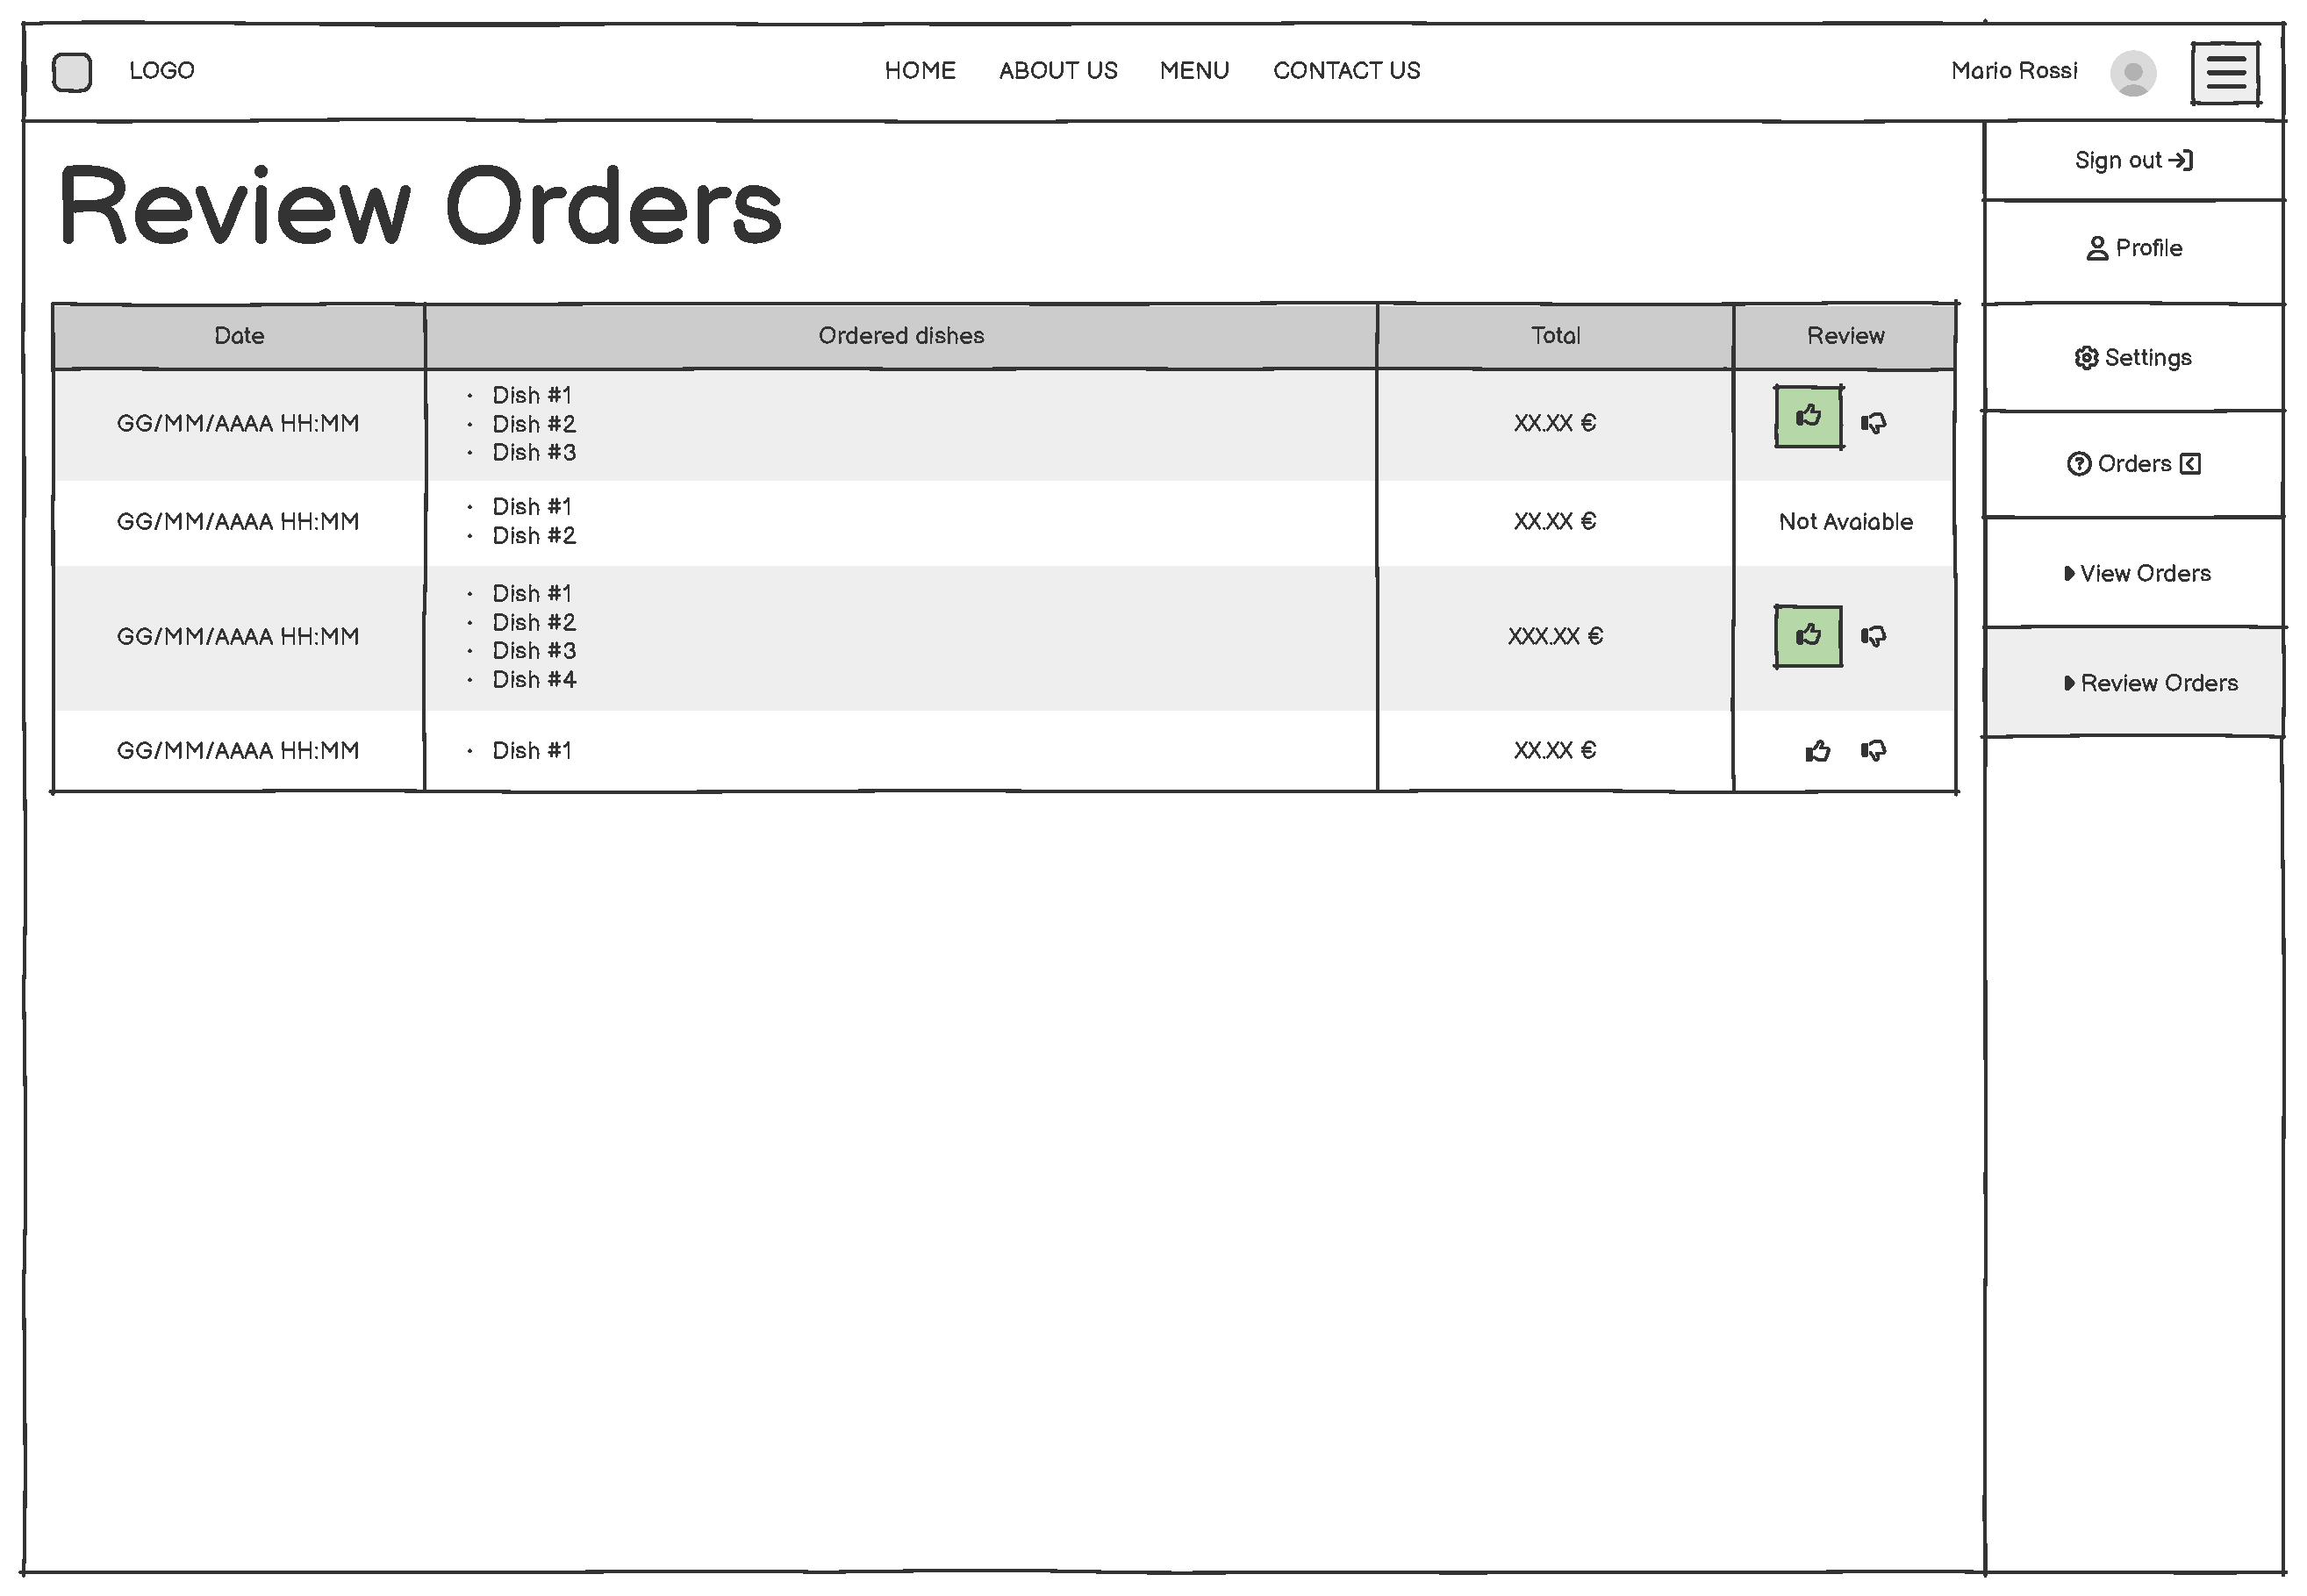
\includegraphics[width=\textwidth]{images/Mockup/ordersReview.pdf}
        \caption{Orders' review mockup page. The order review page gives customers the opportunity to express their opinion on their orders.}
        \label{fig:Orders' review mockup page.}
    \end{subfigure}
    \label{fig:Orders' view customer-side mockup page.}
\end{figure}

\begin{figure}[H]
    \centering
    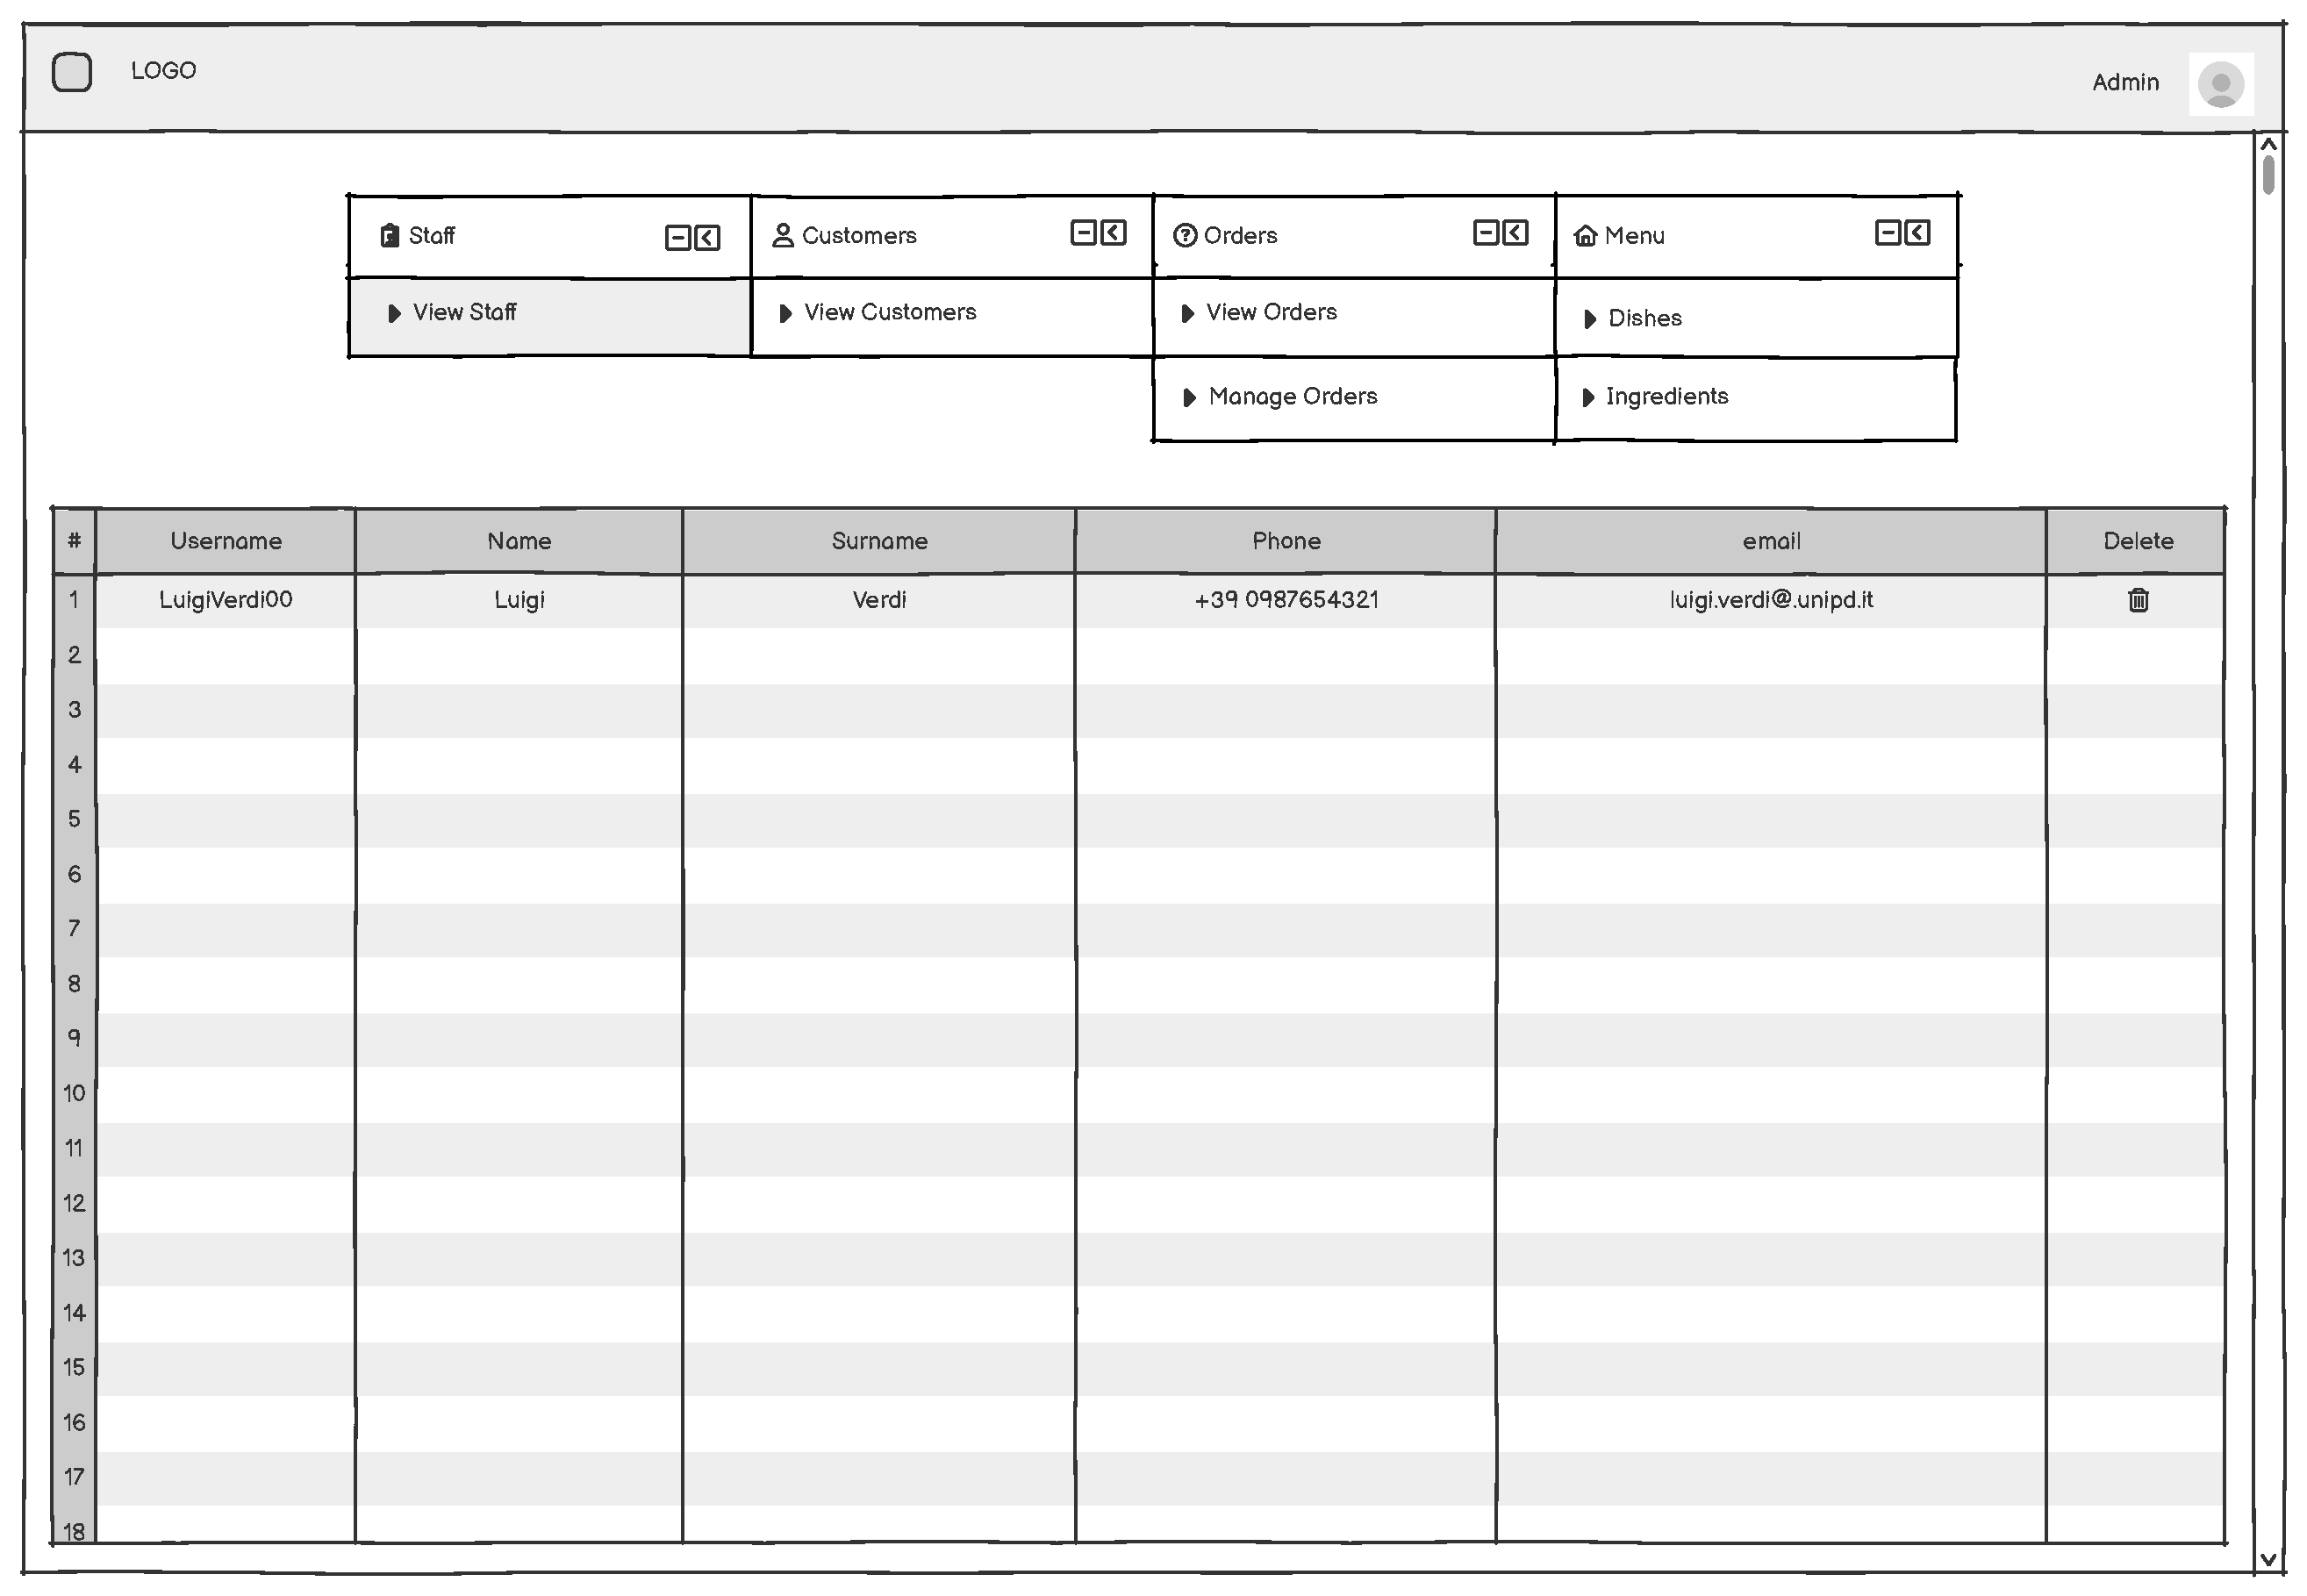
\includegraphics[width=0.55\textwidth]{images/Mockup/staffManagement.pdf}
    \caption{Staff management's mockup page. The staff management page is reserved for administrators and supports the supervision of staff accounts. It represents the interface used to manage internal users.}
    \label{fig:Staff management's mockup page.}
\end{figure}

\begin{figure}[H]
    \centering
    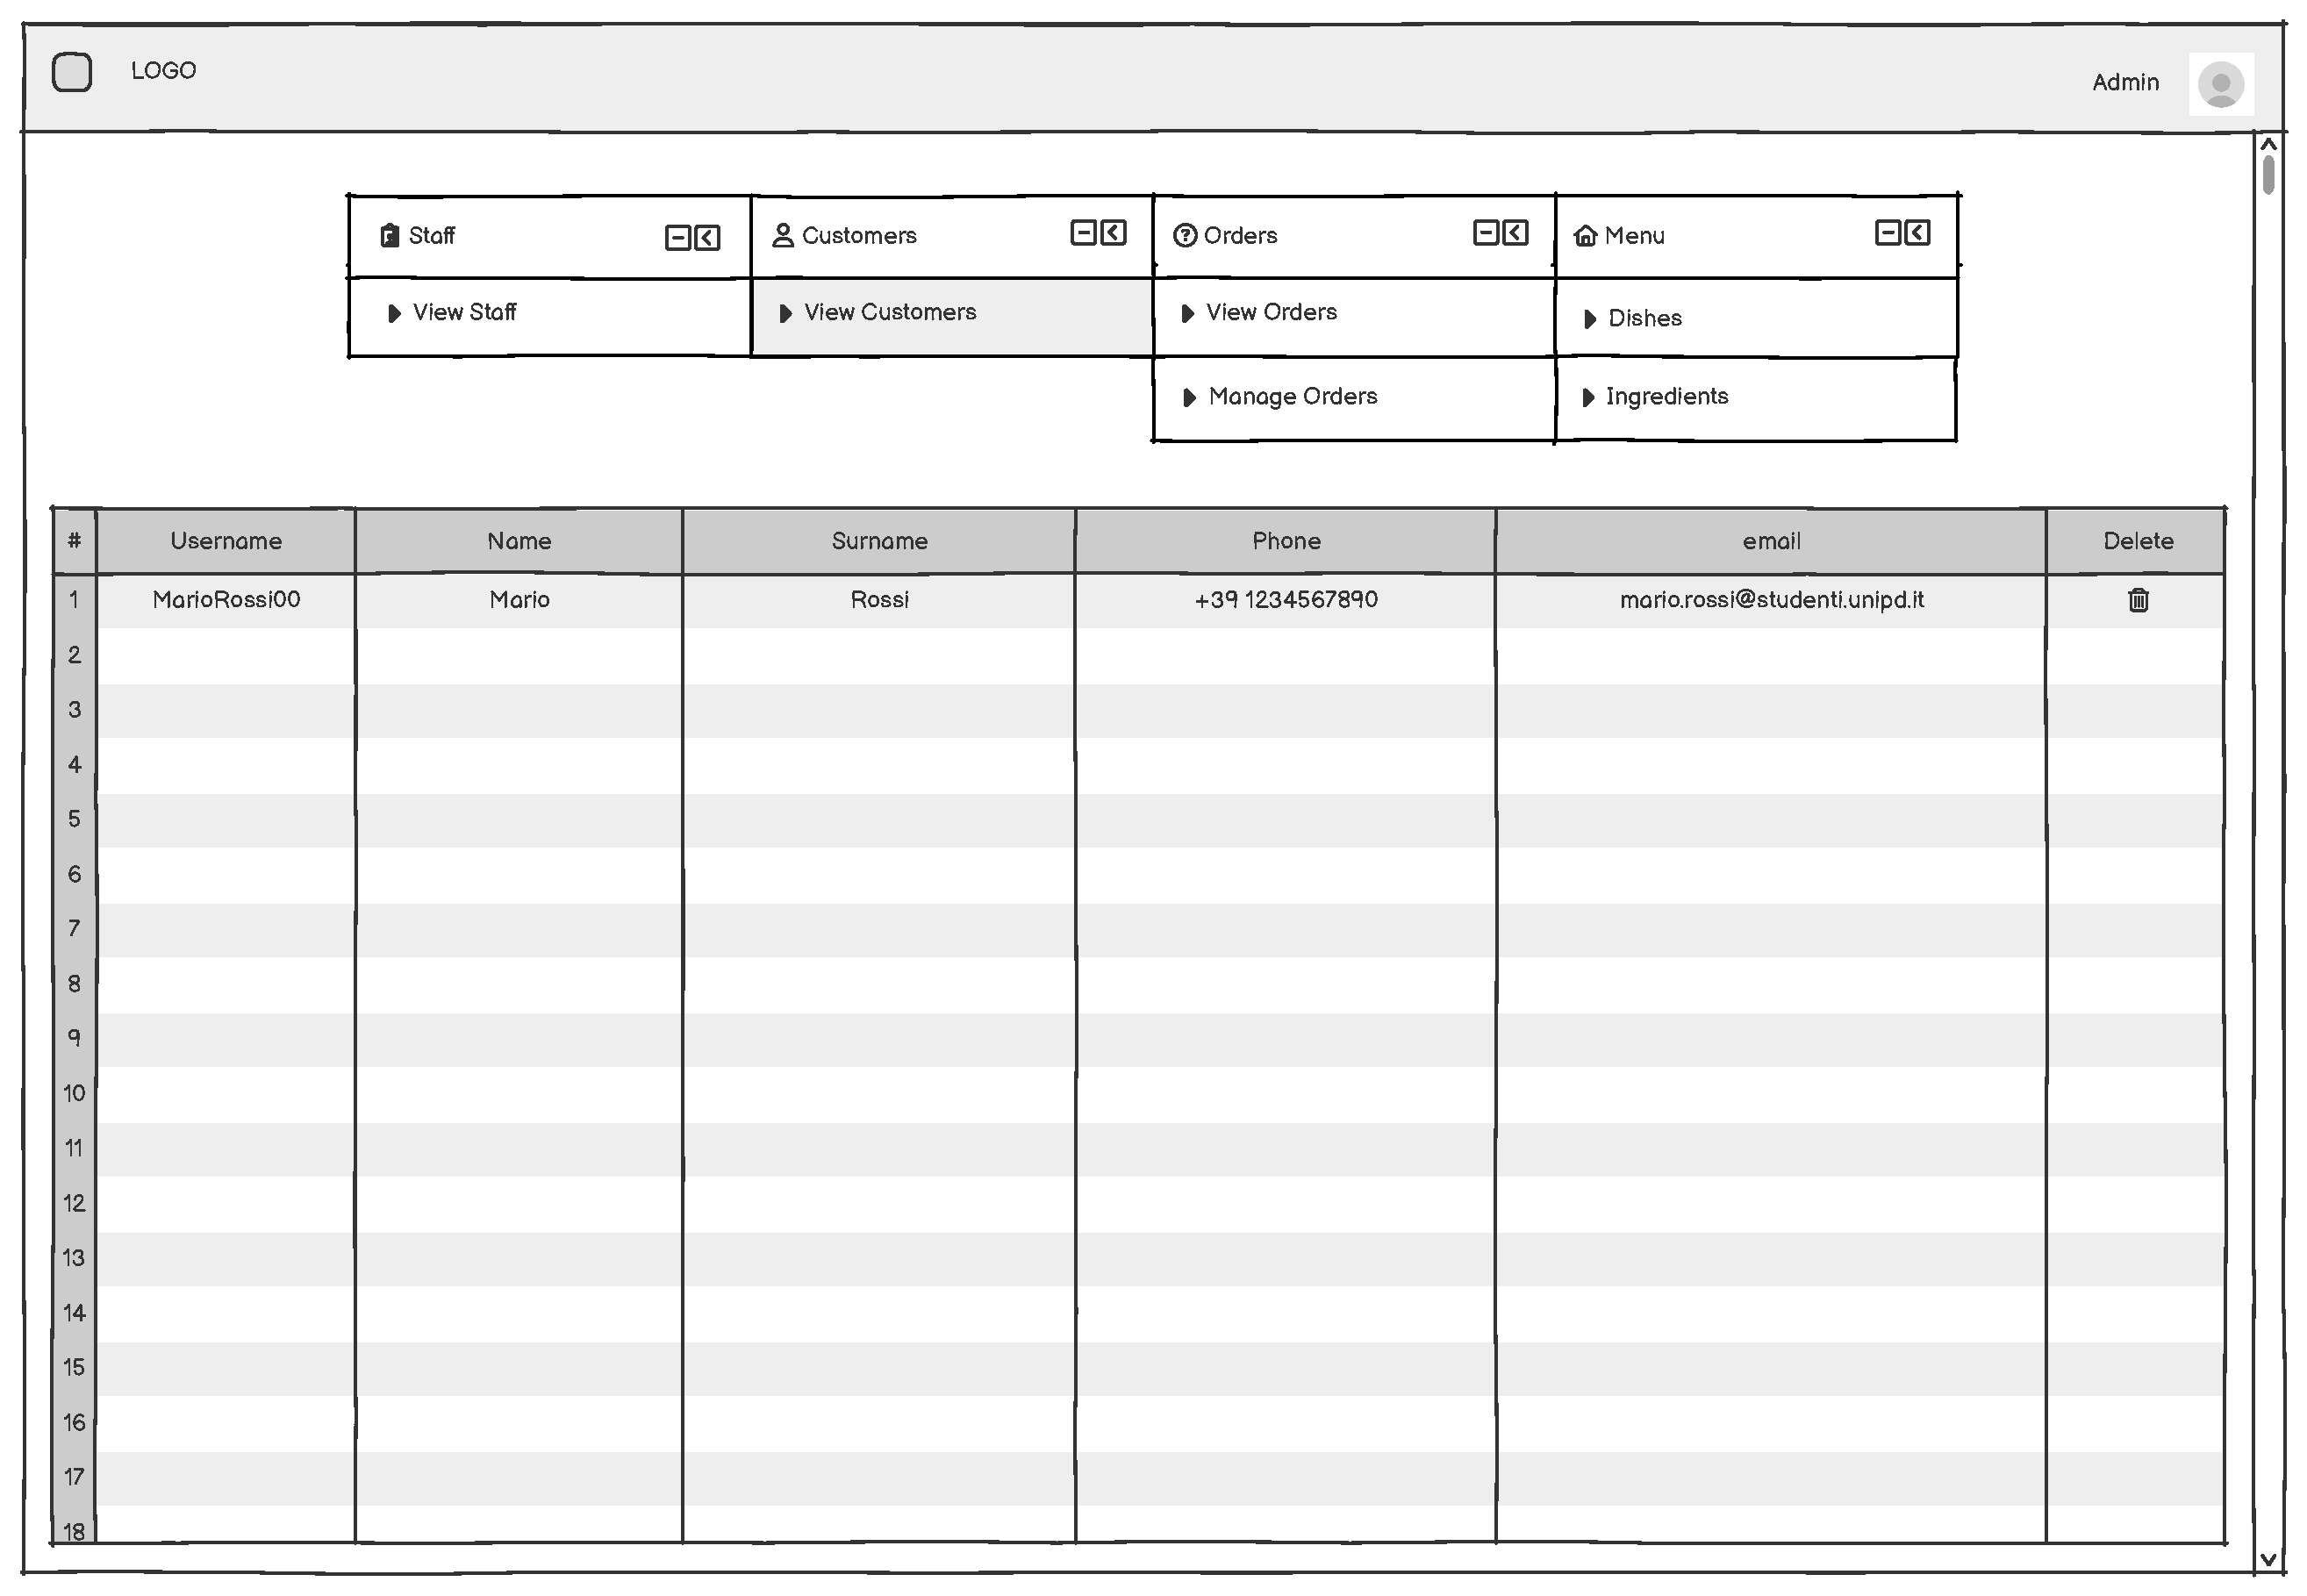
\includegraphics[width=0.55\textwidth]{images/Mockup/customersManagement.pdf}
    \caption{Customers' management mockup page. The customers' management page is intended for administrative users. It provides an overview of registered customers and supports the supervision of customer data from the back-office area.}
    \label{fig:Customers' management mockup page.}
\end{figure}

\begin{figure}[htbp]
    \centering
    \caption{Management status' mockup page.}
    % Prima immagine
    \begin{subfigure}[t]{0.47\textwidth}
        \centering
        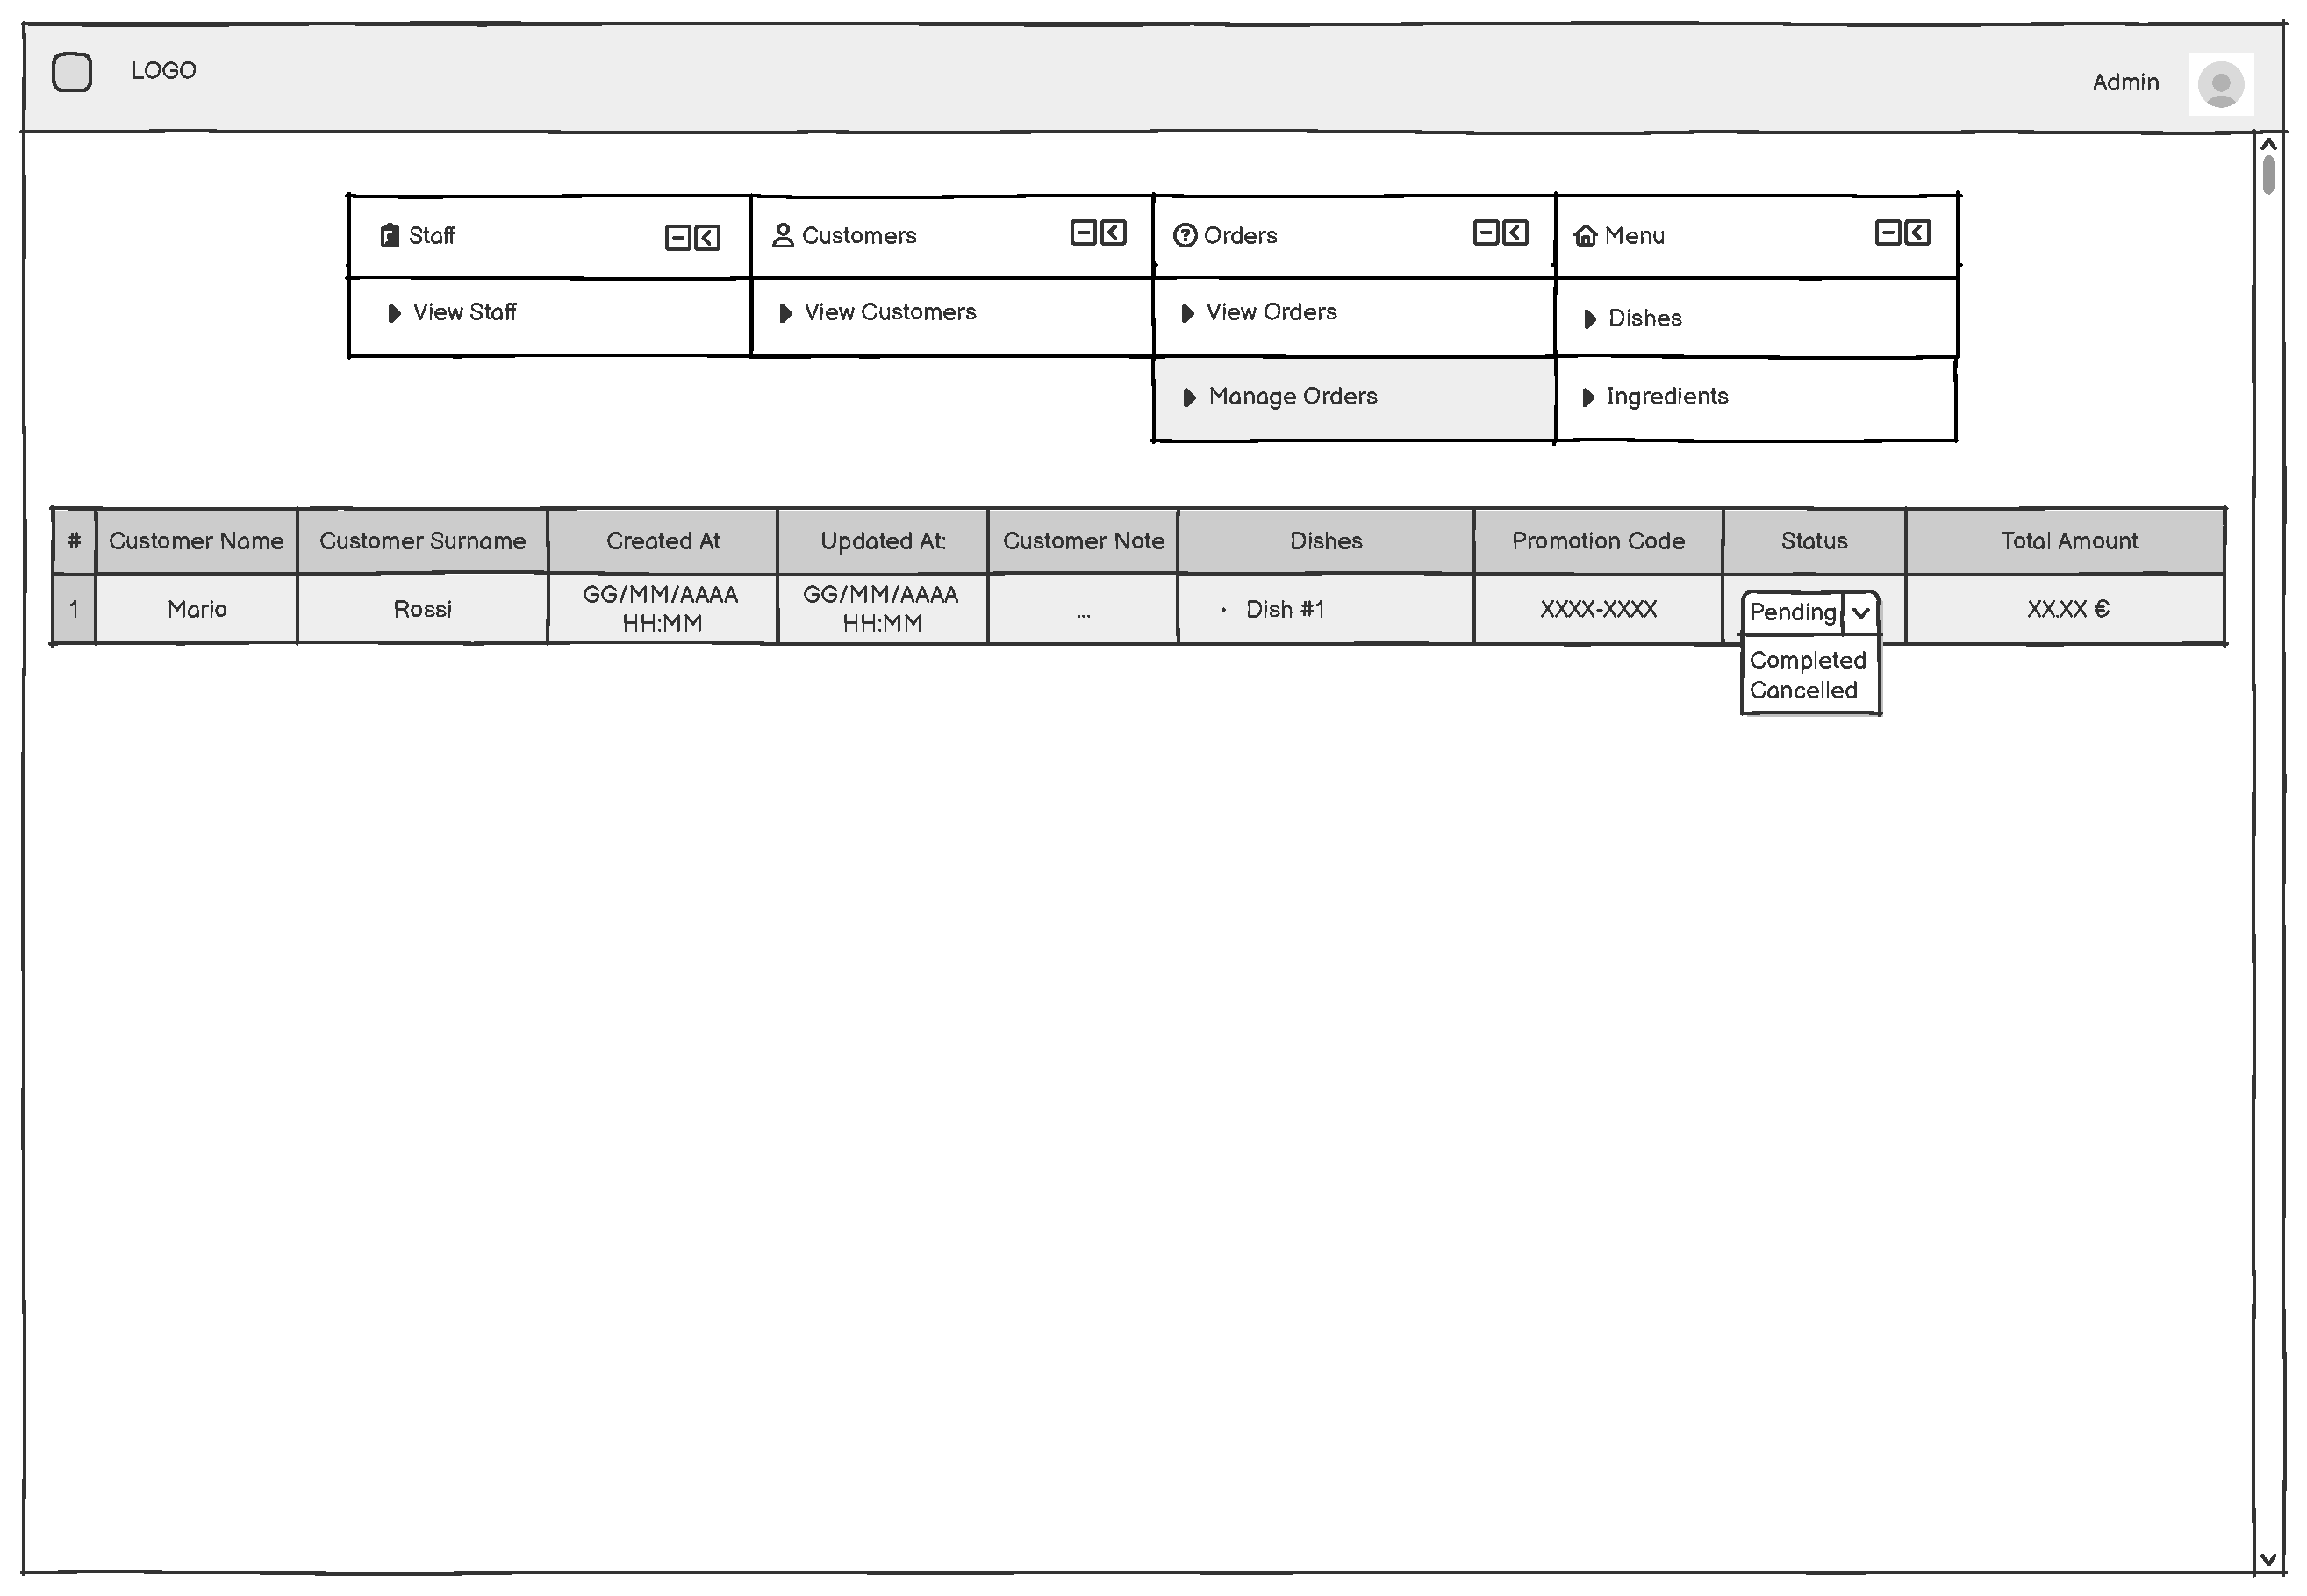
\includegraphics[width=\textwidth]{images/Mockup/adminOrdersManagement.pdf}
        \caption{Management admin-side status' mockup page. The admin-side orders management page gives administrators a global view of order statuses and exposes the controls required to coordinate the order workflow.}
        \label{fig:Management admin-side status' mockup page.}
    \end{subfigure}
    \hfill % Spazio orizzontale tra le immagini
    % Seconda immagine
    \begin{subfigure}[t]{0.47\textwidth}
        \centering
        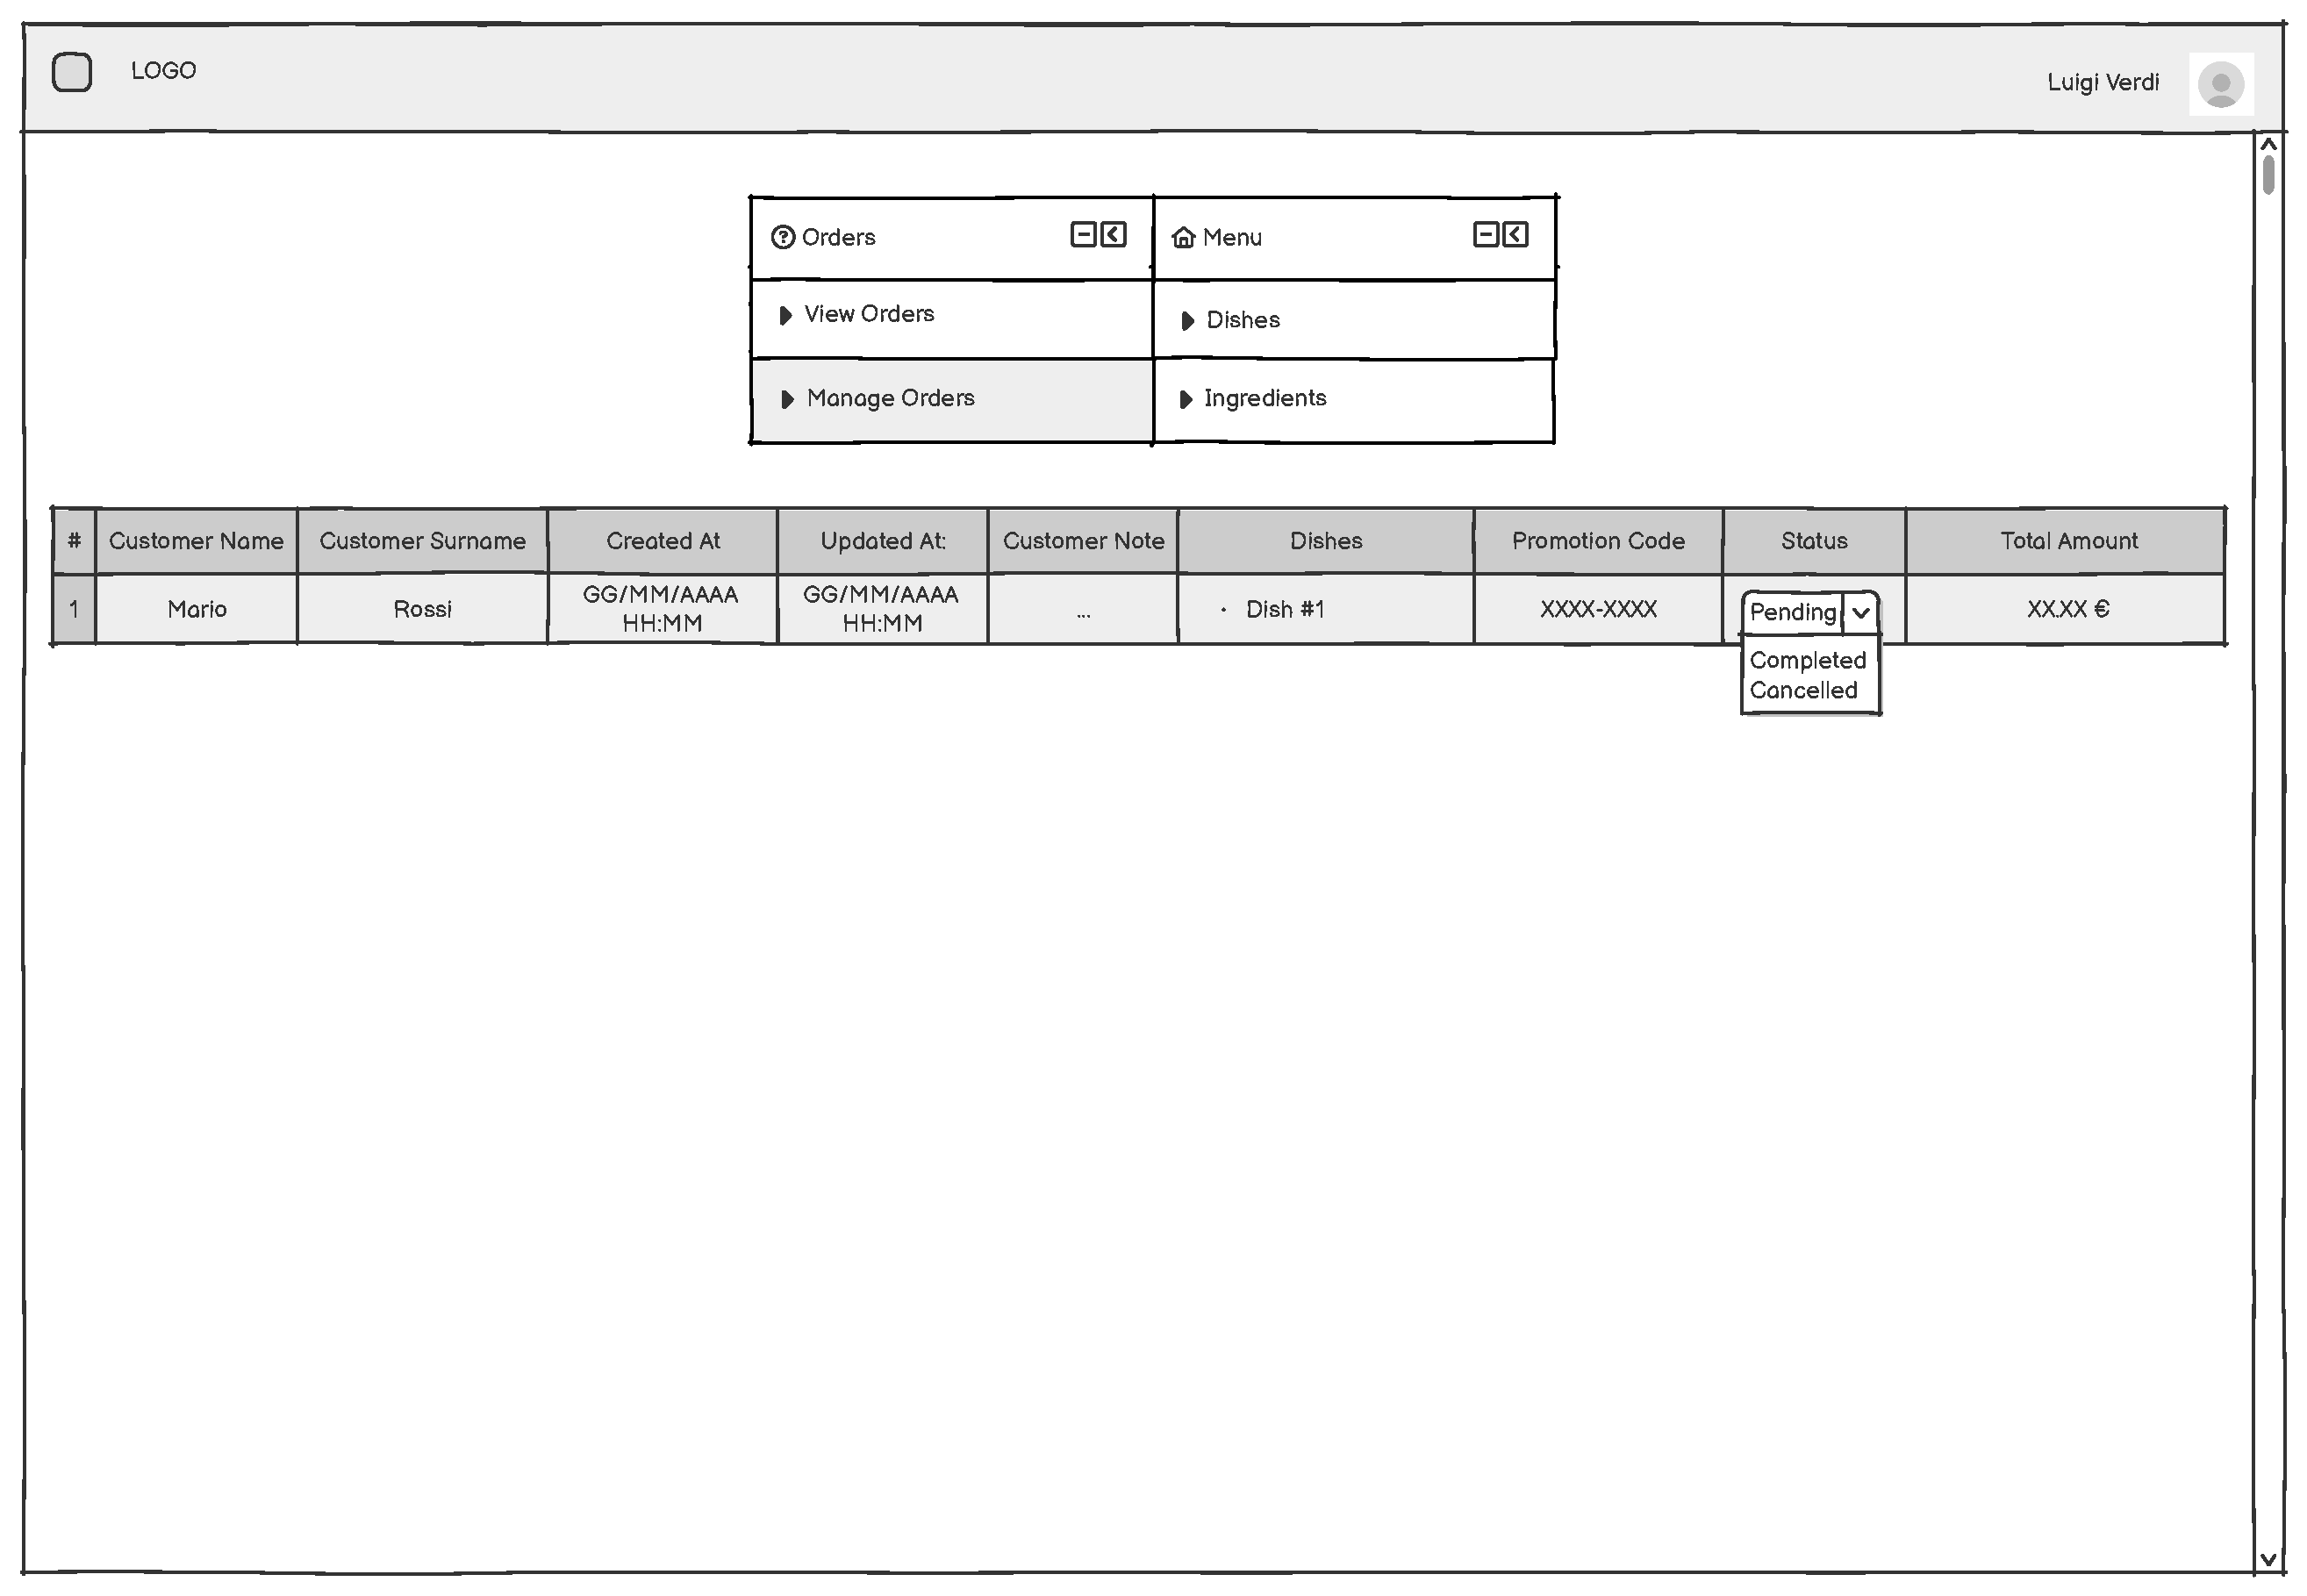
\includegraphics[width=\textwidth]{images/Mockup/staffOrdersManagement.pdf}
        \caption{Management staff-side status' mockup page. The staff-side orders management page focuses on the operational tasks assigned to staff members.}
        \label{fig:Management staff-side status' mockup page.}
    \end{subfigure}
    \label{fig:Management status' mockup page.}
\end{figure}

\begin{figure}[htbp]
    \centering
    \caption{Orders' view admin/staff-side mockup page.}
    % Prima immagine
    \begin{subfigure}[t]{0.47\textwidth}
        \centering
        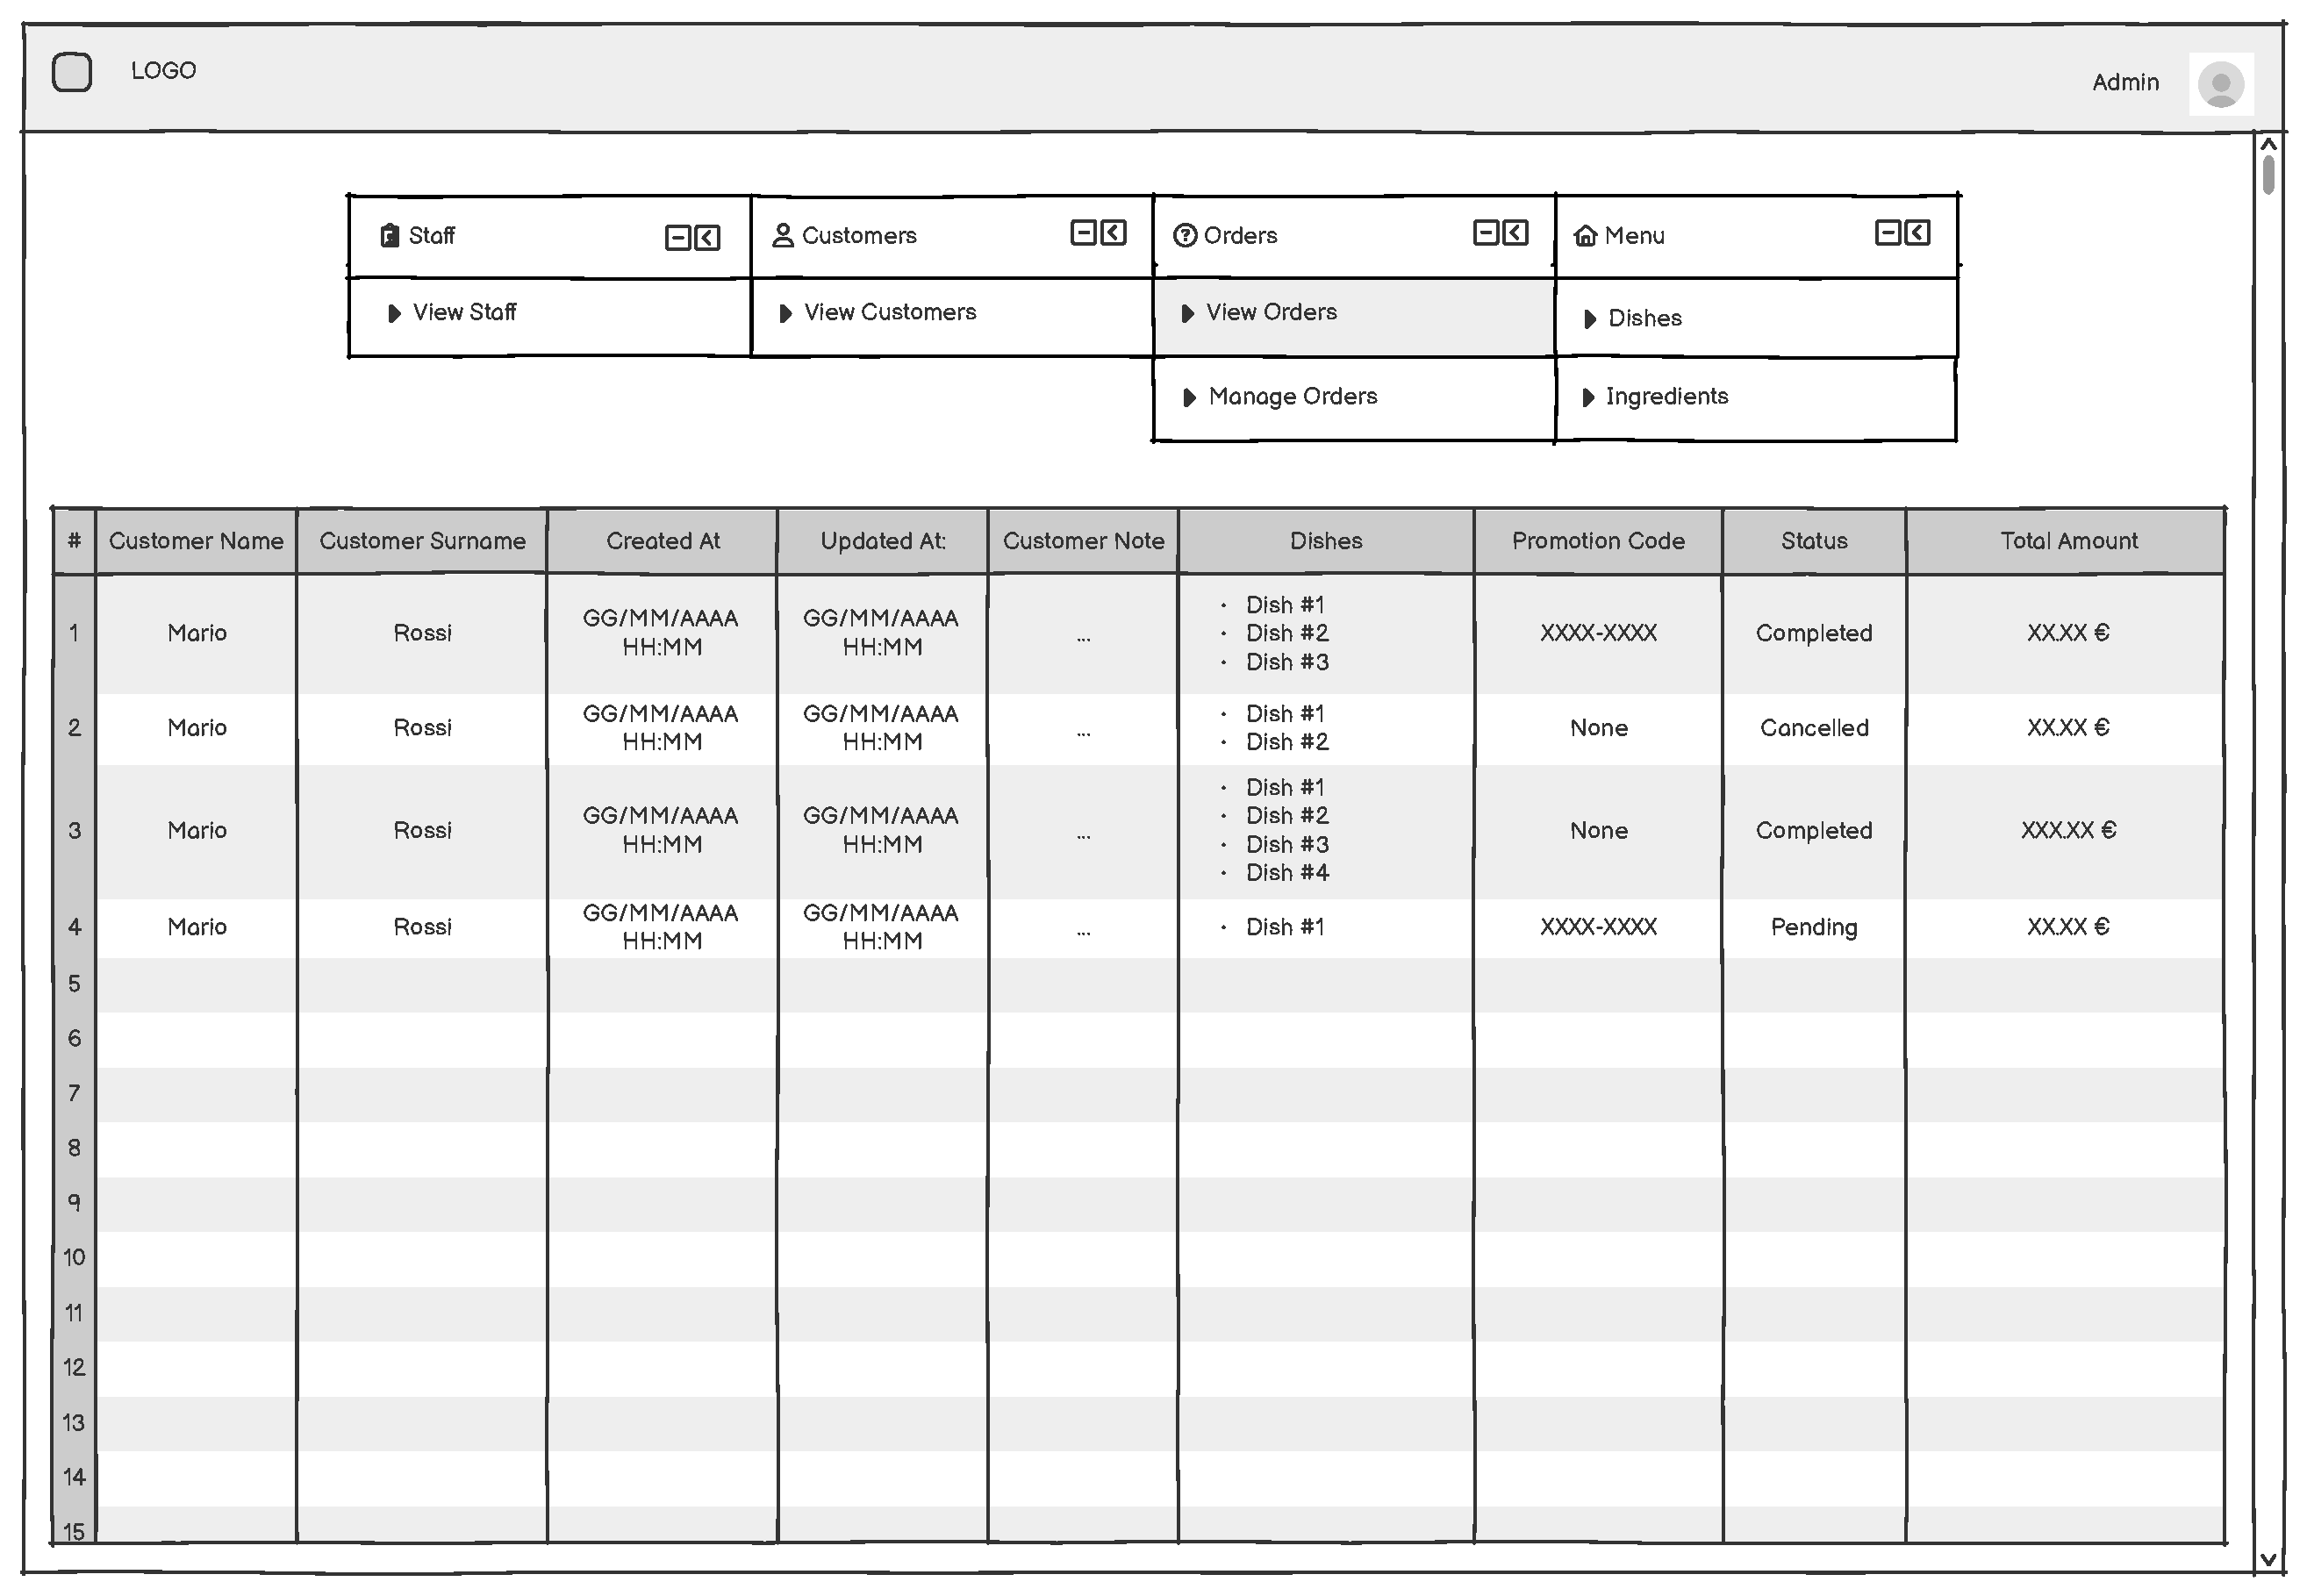
\includegraphics[width=\textwidth]{images/Mockup/adminOrdersView.pdf}
        \caption{Orders' view admin-side mockup page. The admin-side order view page provides detailed information about all orders.}
        \label{fig:Orders' view admin-side mockup page.}
    \end{subfigure}
    \hfill % Spazio orizzontale tra le immagini
    % Seconda immagine
    \begin{subfigure}[t]{0.47\textwidth}
        \centering
        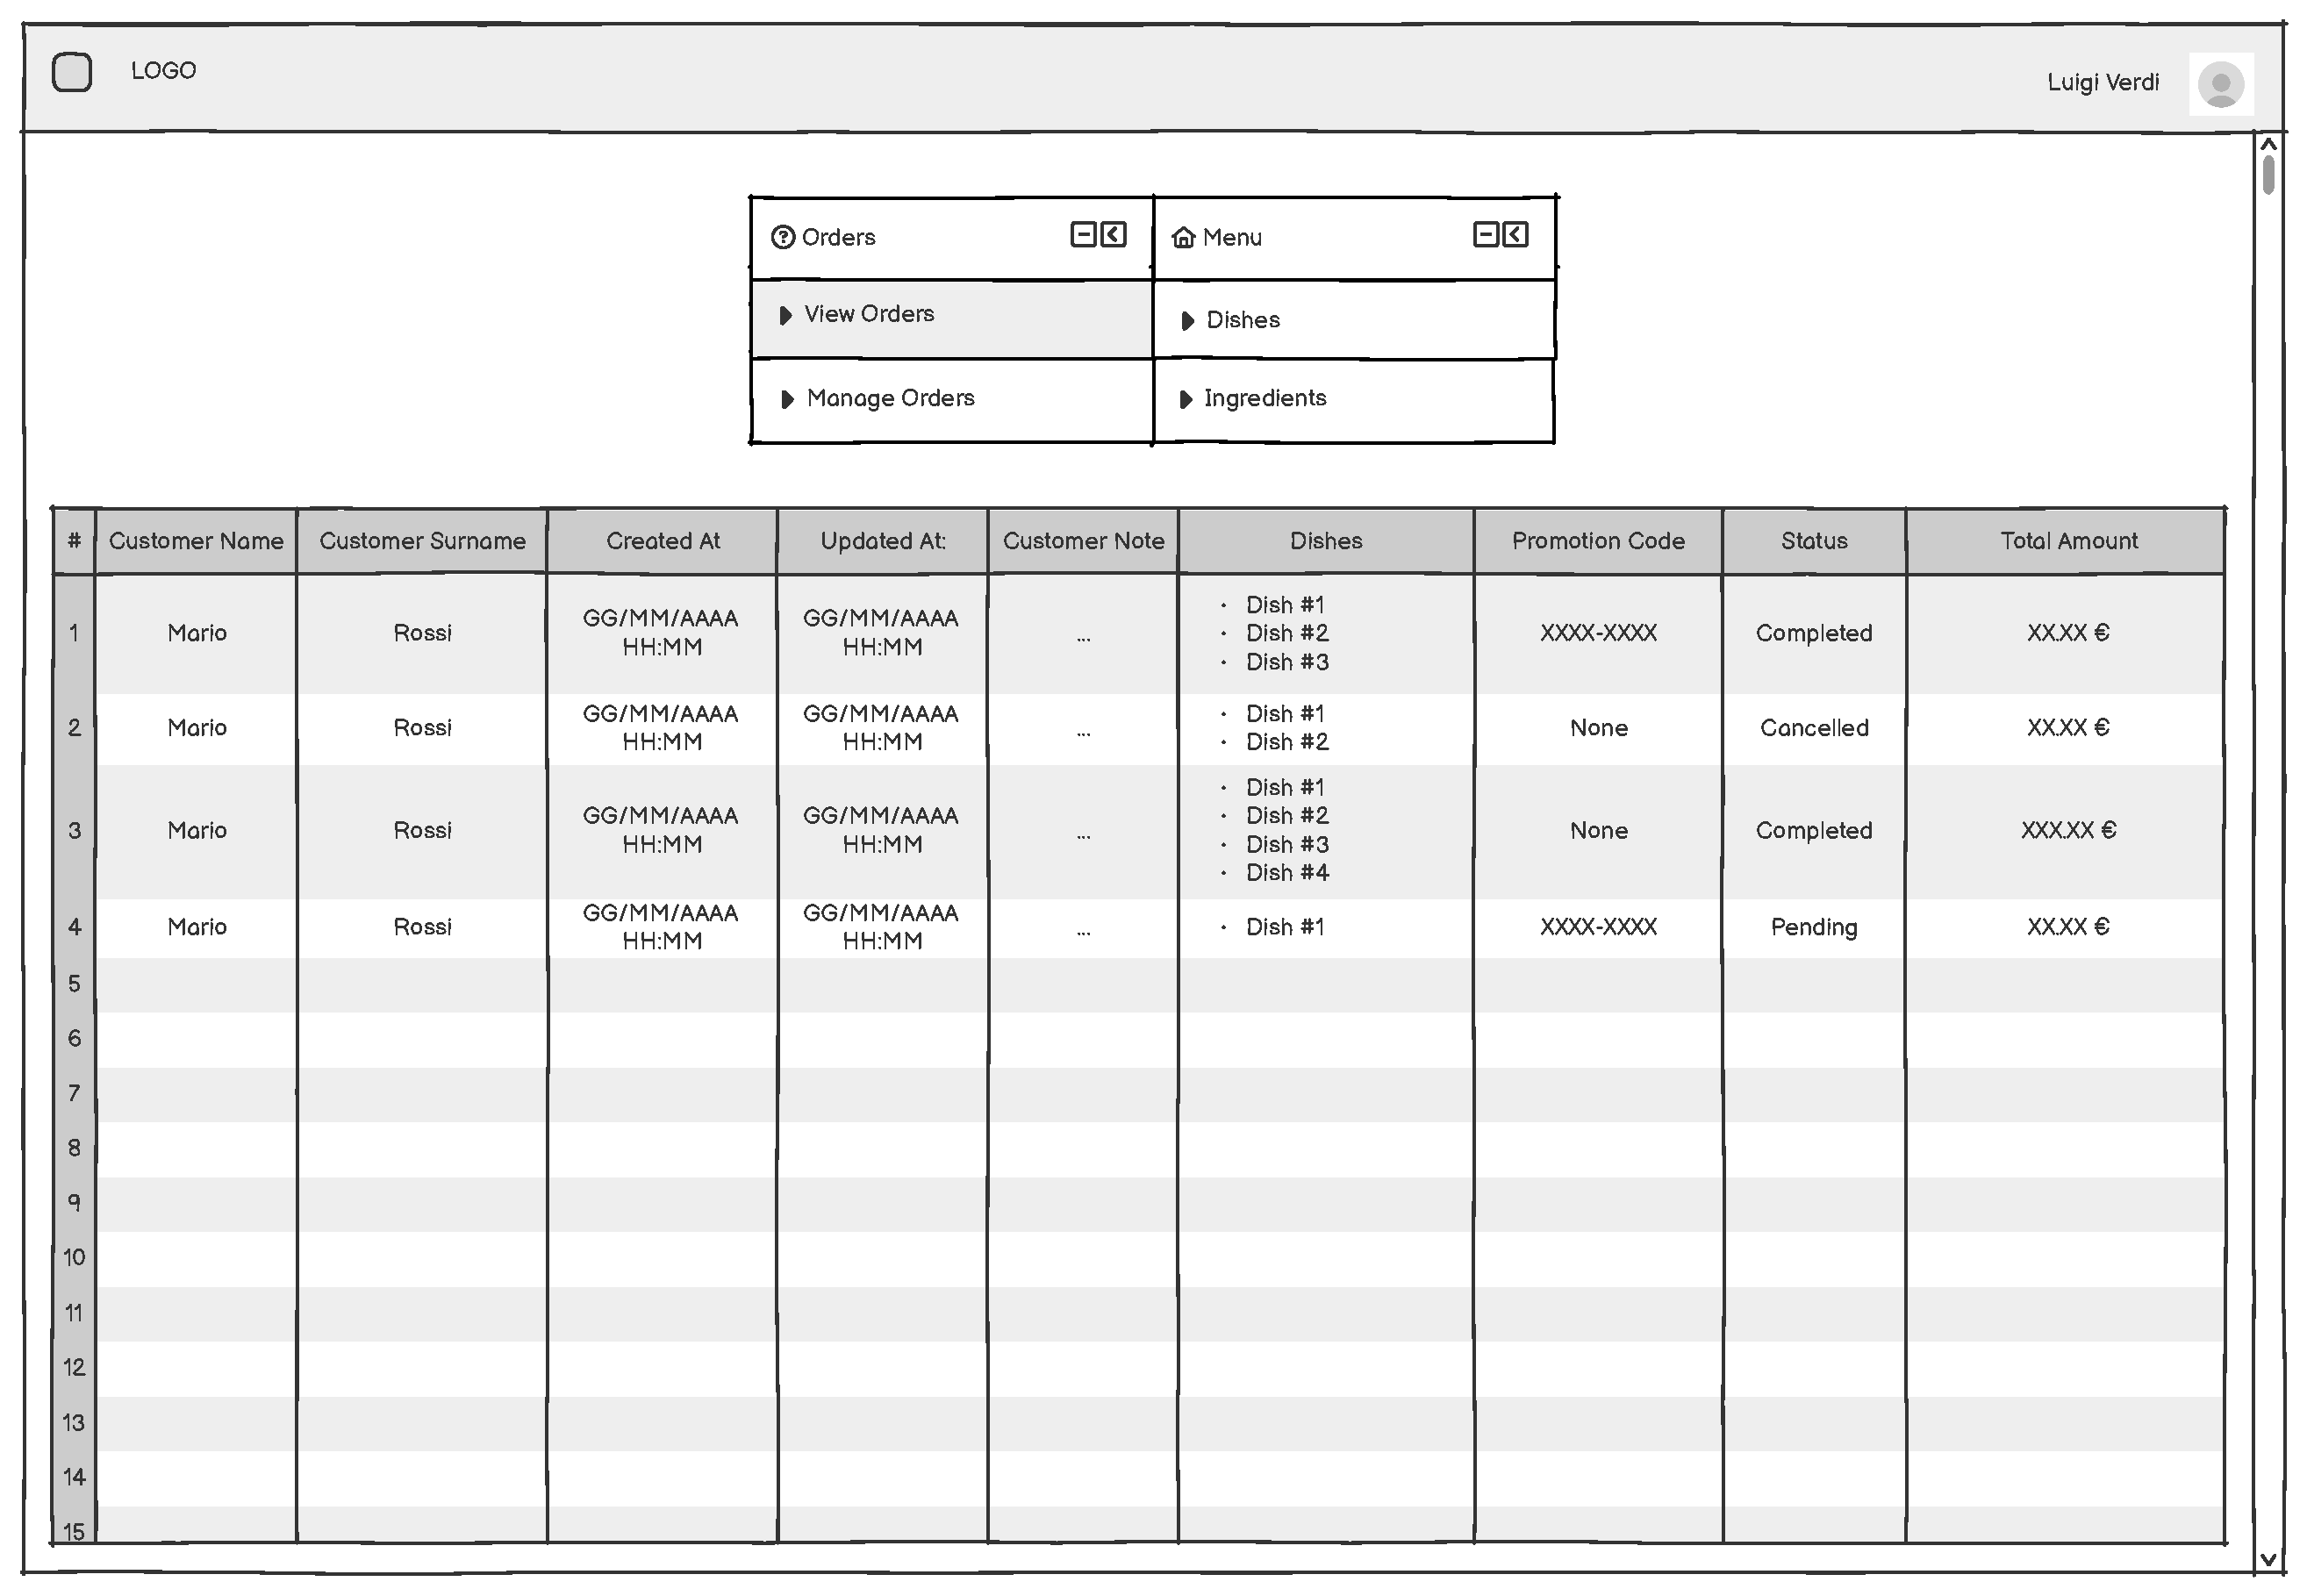
\includegraphics[width=\textwidth]{images/Mockup/staffOrdersView.pdf}
        \caption{Orders' view staff-side mockup page. The staff-side orders view page shows the details needed by staff members to prepare or manage orders.}
        \label{fig:Orders' view staff-side mockup page.}
    \end{subfigure}
    \label{fig:Orders' view admin/staff-side mockup page.}
\end{figure}
